\documentclass[11pt,fleqn, openany]{book} % Default font size and left-justified equations

%%%%%%%%%%%%%%%%%%%%%%%%%%%%%%%%%%%%%%%%%
% The Legrand Orange Book
% Structural Definitions File
% Version 2.1 (26/09/2018)
%
% Original author:
% Mathias Legrand (legrand.mathias@gmail.com) with modifications by:
% Vel (vel@latextemplates.com)
% 
% This file was downloaded from:
% http://www.LaTeXTemplates.com
%
% License:
% CC BY-NC-SA 3.0 (http://creativecommons.org/licenses/by-nc-sa/3.0/)
%
%%%%%%%%%%%%%%%%%%%%%%%%%%%%%%%%%%%%%%%%%

%----------------------------------------------------------------------------------------
%	VARIOUS REQUIRED PACKAGES AND CONFIGURATIONS
%----------------------------------------------------------------------------------------

\usepackage[table]{xcolor}

\usepackage{graphicx}
\usepackage{tabularx} % Required for including pictures
\usepackage{pgf,tikz,tkz-tab,eurosym,yhmath, stmaryrd}
\usepackage{pgfplots}
\usepackage{mathrsfs}
\usetikzlibrary{patterns}
\usetikzlibrary{trees}
\graphicspath{{../../Pictures/}}
\usepackage{multicol} 


\usepackage[english]{babel} % English language/hyphenation
\usepackage{icomma}
\usepackage{enumitem} % Customize lists
\setlist{nolistsep, nosep, nolistsep} % Reduce spacing between bullet points and numbered lists

\usepackage{booktabs} % Required for nicer horizontal rules in tables

 % Required for specifying colors by name


\definecolor{ocre}{RGB}{243,102,25} % Define the orange color used for highlighting throughout the book

\usepackage{listings}

\definecolor{codegreen}{rgb}{0,0.6,0}
\definecolor{codegray}{rgb}{0.5,0.5,0.5}
\definecolor{codepurple}{rgb}{0.58,0,0.82}
\definecolor{backcolour}{rgb}{0.95,0.95,0.92}

\lstdefinestyle{mystyle}{
    backgroundcolor=\color{backcolour},   
    commentstyle=\color{codegreen},
    keywordstyle=\color{magenta},
    numberstyle=\tiny\color{codegray},
    stringstyle=\color{codepurple},
    basicstyle=\ttfamily\footnotesize,
    breakatwhitespace=false,         
    breaklines=true,                 
    captionpos=b,                    
    keepspaces=true,                 
    numbers=left,                    
    numbersep=5pt,                  
    showspaces=false,                
    showstringspaces=false,
    showtabs=false,                  
    tabsize=2
}

\lstset{style=mystyle}

%----------------------------------------------------------------------------------------
% Paramétrage XSIM
%----------------------------------------------------------------------------------------

\usepackage[no-files]{xsim}


\DeclareExerciseEnvironmentTemplate{myex}{%
    \textbf{%
      \hypertarget{ex:\ExerciseID}{\sffamily{\ensuremath{\blacktriangleright}} Exercice \GetExerciseProperty{counter} \GetExerciseProperty{subtitle} --}
      \hyperlink{sol:\ExerciseID}{Voir le corrigé}%
    }\par
}{\par\smallskip}

\DeclareExerciseEnvironmentTemplate{mysol}{%
    \textbf{%
      \hypertarget{sol:\ExerciseID}{\sffamily{\ensuremath{\blacktriangleright}} Correction \GetExerciseProperty{counter} --}
      \hyperlink{ex:\ExerciseID}{Voir l'énoncé}%
    }\par
}{\par\medskip}

\xsimsetup{
  exercise/template = myex ,
  solution/template = mysol 
}

%Collection exercices

\DeclareExerciseTagging{topic}

\xsimsetup{collect}

%----------------------------------------------------------------------------------------
% SYMBOLES
%----------------------------------------------------------------------------------------

\newcommand\imCMsym[4][\mathord]{%
  \DeclareFontFamily{U} {#2}{}
  \DeclareFontShape{U}{#2}{m}{n}{
    <-6> #25
    <6-7> #26
    <7-8> #27
    <8-9> #28
    <9-10> #29
    <10-12> #210
    <12-> #212}{}
  \DeclareSymbolFont{CM#2} {U} {#2}{m}{n}
  \DeclareMathSymbol{#4}{#1}{CM#2}{#3}
}
\newcommand\alsoimCMsym[4][\mathord]{\DeclareMathSymbol{#4}{#1}{CM#2}{#3}}

\imCMsym{cmmi}{124}{\CMjmath}

\newcommand{\Oij}{(O\,;\,\vec{\imath}\,,\, \vec{\CMjmath} )}
\newcommand{\Oijk}{(O\,;\,\vec{\imath}\,,\, \vec{\CMjmath}\,,\,\vec{k})}

\newcommand\e{\mathrm{e}}
\newcommand\R{\mathbb{R}}
\newcommand\N{\mathbb{N}}


%----------------------------------------------------------------------------------------
%	MARGINS
%----------------------------------------------------------------------------------------

\usepackage{geometry} % Required for adjusting page dimensions and margins

\geometry{
	paper=a4paper, % Paper size, change to letterpaper for US letter size
	top=3cm, % Top margin
	bottom=3cm, % Bottom margin
	left=2cm, % Left margin
	right=2cm, % Right margin
	headheight=14pt, % Header height
	footskip=1.4cm, % Space from the bottom margin to the baseline of the footer
	headsep=10pt, % Space from the top margin to the baseline of the header
	%showframe, % Uncomment to show how the type block is set on the page
}

\setlength{\parindent}{0pt}
\parskip=5pt



%----------------------------------------------------------------------------------------
%	FONTS
%----------------------------------------------------------------------------------------

\usepackage{avant} % Use the Avantgarde font for headings
\usepackage{times} % Use the Times font for headings
\usepackage{mathptmx} % Use the Adobe Times Roman as the default text font together with math symbols from the Sym­bol, Chancery and Com­puter Modern fonts

%\usepackage{microtype} % Slightly tweak font spacing for aesthetics
%\usepackage[utf8]{inputenc} % Required for including letters with accents
\usepackage[T1]{fontenc} % Use 8-bit encoding that has 256 glyphs

%----------------------------------------------------------------------------------------
%	BIBLIOGRAPHY AND INDEX
%----------------------------------------------------------------------------------------

\usepackage[style=numeric,citestyle=numeric,sorting=nyt,sortcites=true,autopunct=true,babel=hyphen,hyperref=true,abbreviate=false,backref=true,backend=biber]{biblatex}
\addbibresource{bibliography.bib} % BibTeX bibliography file
\defbibheading{bibempty}{}

\usepackage{calc} % For simpler calculation - used for spacing the index letter headings correctly
\usepackage{makeidx} % Required to make an index
\makeindex % Tells LaTeX to create the files required for indexing

%----------------------------------------------------------------------------------------
%	MAIN TABLE OF CONTENTS
%----------------------------------------------------------------------------------------

\usepackage{titletoc} % Required for manipulating the table of contents

\contentsmargin{0cm} % Removes the default margin

% Part text styling (this is mostly taken care of in the PART HEADINGS section of this file)
\titlecontents{part}
	[0cm] % Left indentation
	{\addvspace{20pt}\bfseries} % Spacing and font options for parts
	{}
	{}
	{}

% Chapter text styling
\titlecontents{chapter}
	[1.25cm] % Left indentation
	{\addvspace{12pt}\large\sffamily\bfseries} % Spacing and font options for chapters
	{\color{ocre!60}\contentslabel[\Large\thecontentslabel]{1.25cm}\color{ocre}} % Formatting of numbered sections of this type
	{\color{ocre}} % Formatting of numberless sections of this type
	{\color{ocre!60}\normalsize\;\titlerule*[.5pc]{.}\;\thecontentspage} % Formatting of the filler to the right of the heading and the page number

% Section text styling
\titlecontents{section}
	[1.25cm] % Left indentation
	{\addvspace{3pt}\sffamily\bfseries} % Spacing and font options for sections
	{\contentslabel[\thecontentslabel]{1.25cm}} % Formatting of numbered sections of this type
	{} % Formatting of numberless sections of this type
	{\hfill\color{black}\thecontentspage} % Formatting of the filler to the right of the heading and the page number

% Subsection text styling
\titlecontents{subsection}
	[1.25cm] % Left indentation
	{\addvspace{1pt}\sffamily\small} % Spacing and font options for subsections
	{\contentslabel[\thecontentslabel]{1.25cm}} % Formatting of numbered sections of this type
	{} % Formatting of numberless sections of this type
	{\ \titlerule*[.5pc]{.}\;\thecontentspage} % Formatting of the filler to the right of the heading and the page number

% Figure text styling
\titlecontents{figure}
	[1.25cm] % Left indentation
	{\addvspace{1pt}\sffamily\small} % Spacing and font options for figures
	{\thecontentslabel\hspace*{1em}} % Formatting of numbered sections of this type
	{} % Formatting of numberless sections of this type
	{\ \titlerule*[.5pc]{.}\;\thecontentspage} % Formatting of the filler to the right of the heading and the page number

% Table text styling
\titlecontents{table}
	[1.25cm] % Left indentation
	{\addvspace{1pt}\sffamily\small} % Spacing and font options for tables
	{\thecontentslabel\hspace*{1em}} % Formatting of numbered sections of this type
	{} % Formatting of numberless sections of this type
	{\ \titlerule*[.5pc]{.}\;\thecontentspage} % Formatting of the filler to the right of the heading and the page number

%----------------------------------------------------------------------------------------
%	MINI TABLE OF CONTENTS IN PART HEADS
%----------------------------------------------------------------------------------------

% Chapter text styling
\titlecontents{lchapter}
	[0em] % Left indentation
	{\addvspace{15pt}\large\sffamily\bfseries} % Spacing and font options for chapters
	{\color{ocre}\contentslabel[\Large\thecontentslabel]{1.25cm}\color{ocre}} % Chapter number
	{}  
	{\color{ocre}\normalsize\sffamily\bfseries\;\titlerule*[.5pc]{.}\;\thecontentspage} % Page number

% Section text styling
\titlecontents{lsection}
	[0em] % Left indentation
	{\sffamily\small} % Spacing and font options for sections
	{\contentslabel[\thecontentslabel]{1.25cm}} % Section number
	{}
	{}

% Subsection text styling (note these aren't shown by default, display them by searchings this file for tocdepth and reading the commented text)
\titlecontents{lsubsection}
	[.5em] % Left indentation
	{\sffamily\footnotesize} % Spacing and font options for subsections
	{\contentslabel[\thecontentslabel]{1.25cm}}
	{}
	{}

%----------------------------------------------------------------------------------------
%	HEADERS AND FOOTERS
%----------------------------------------------------------------------------------------


\usepackage{fancyhdr} % Required for header and footer configuration

\pagestyle{fancy}
\renewcommand{\chaptermark}[1]{\markboth{\sffamily\normalsize\bfseries\ \thechapter.\ #1}{}} % Chapter text font settings
\renewcommand{\sectionmark}[1]{\markright{\sffamily\normalsize\thesection\hspace{5pt}#1}{}} % Section text font settings
\fancyhf{} \fancyhead[LE,RO]{\sffamily\normalsize\thepage} % Font setting for the page number in the header
\fancyhead[LO]{\rightmark} % Print the nearest section name on the left side of odd pages
\fancyhead[RE]{\leftmark} % Print the current chapter name on the right side of even pages

\fancyfoot[L]{Jason LAPEYRONNIE}
\fancyfoot[R]{\href{http://mathoutils.fr}{http://mathoutils.fr}} % Uncomment to include a footer

\renewcommand{\headrulewidth}{0.5pt} % Thickness of the rule under the header
\renewcommand{\footrulewidth}{0.5pt} % Thickness of the rule under the header

\fancypagestyle{plain}{% Style for when a plain pagestyle is specified
	\fancyhead{}\renewcommand{\headrulewidth}{0pt}%
}

% Removes the header from odd empty pages at the end of chapters
\makeatletter
\renewcommand{\cleardoublepage}{
\clearpage\ifodd\c@page\else
\hbox{}
\vspace*{\fill}
\thispagestyle{empty}
\newpage
\fi}

%----------------------------------------------------------------------------------------
%	THEOREM STYLES
%----------------------------------------------------------------------------------------

\usepackage{amsmath,amsfonts,amssymb,amsthm} % For math equations, theorems, symbols, etc

\newcommand{\intoo}[2]{\mathopen{]}#1\,;#2\mathclose{[}}
\newcommand{\ud}{\mathop{\mathrm{{}d}}\mathopen{}}
\newcommand{\intff}[2]{\mathopen{[}#1\,;#2\mathclose{]}}
\renewcommand{\qedsymbol}{$\blacksquare$}
\newtheorem{notation}{Notation}[section]

% Boxed/framed environments
\newtheoremstyle{ocrenumbox}% Theorem style name
{0pt}% Space above
{0pt}% Space below
{\normalfont}% Body font
{}% Indent amount
{\small\bf\sffamily\color{ocre}}% Theorem head font
{\;:\;}% Punctuation after theorem head
{0.25em}% Space after theorem head
{\small\sffamily\color{ocre}\thmname{#1}\nobreakspace\thmnumber{\@ifnotempty{#1}{}\@upn{#2}}% Theorem text (e.g. Theorem 2.1)
\thmnote{\nobreakspace\the\thm@notefont\sffamily\bfseries\color{black}---\nobreakspace#3}} % Optional theorem note

\newtheoremstyle{blacknumex}% Theorem style name
{5pt}% Space above
{10pt}% Space below
{\normalfont}% Body font
{} % Indent amount
{\small\bf\sffamily}% Theorem head font
{\;:\;}% Punctuation after theorem head
{0.25em}% Space after theorem head
{\small\sffamily{\tiny\ensuremath{\blacksquare}}\nobreakspace\thmname{#1}\nobreakspace\thmnumber{\@ifnotempty{#1}{}\@upn{#2}}% Theorem text (e.g. Theorem 2.1)
\thmnote{\nobreakspace\the\thm@notefont\sffamily\bfseries---\nobreakspace#3}}% Optional theorem note

\newtheoremstyle{blacknumexo}% Theorem style name
{15pt}% Space above
{10pt}% Space below
{\normalfont}% Body font
{} % Indent amount
{\small\bf\sffamily}% Theorem head font
{}% Punctuation after theorem head
{0.5em}% Space after theorem head
{\small\sffamily{\ensuremath{\blacktriangleright}}\nobreakspace\thmname{#1}\nobreakspace\thmnumber{\@ifnotempty{#1}{}\@upn{#2}}% Theorem text (e.g. Theorem 2.1)
\thmnote{\nobreakspace\the\thm@notefont\sffamily\bfseries---\nobreakspace#3} \\}% Optional theorem note



\newtheoremstyle{blacknumbox} % Theorem style name
{0pt}% Space above
{5pt}% Space below
{}% Body font
{}% Indent amount
{\large\bf\sffamily}% Theorem head font
{\;:\;}% Punctuation after theorem head
{0.25em}% Space after theorem head
{\small\sffamily\thmname{#1}\nobreakspace\thmnumber{\@ifnotempty{#1}{}\@upn{#2}}% Theorem text (e.g. Theorem 2.1)
\thmnote{\nobreakspace\the\thm@notefont\sffamily\bfseries---\nobreakspace#3}}% Optional theorem note

% Non-boxed/non-framed environments
\newtheoremstyle{ocrenum}% Theorem style name
{5pt}% Space above
{5pt}% Space below
{\normalfont}% Body font
{}% Indent amount
{\small\bf\sffamily\color{ocre}}% Theorem head font
{\;:\;}% Punctuation after theorem head
{0.25em}% Space after theorem head
{\small\sffamily\color{ocre}\thmname{#1}\nobreakspace\thmnumber{\@ifnotempty{#1}{}\@upn{#2}}% Theorem text (e.g. Theorem 2.1)
\thmnote{\nobreakspace\the\thm@notefont\sffamily\bfseries\color{black}---\nobreakspace#3}} % Optional theorem note
\makeatother

% Defines the theorem text style for each type of theorem to one of the three styles above
\newcounter{dummy} 
\newcounter{thm}
\newcounter{correction}
\newcounter{qst}
\theoremstyle{ocrenumbox}
\newtheorem{theoremeT}[dummy]{Théorème}
\newtheorem{exerciseT}{Propriété}
\newtheorem{principeT}{Principe}
\theoremstyle{blacknumex}
\newtheorem{exampleT}{Exemple}
\theoremstyle{blacknumexo}
\newtheorem{exo}[thm]{Exercice}
\newtheorem{corr}[correction]{Correction}
\newtheorem{quest}[qst]{Question}
\theoremstyle{blacknumbox}
\newtheorem{vocabulary}{Vocabulary}[section]
\newtheorem{definitionT}{Définition}
\newtheorem{corollaryT}[dummy]{Corollary}
\theoremstyle{ocrenum}
\newtheorem{proofT}[dummy]{Démonstration}


%----------------------------------------------------------------------------------------
%	DEFINITION OF COLORED BOXES
%----------------------------------------------------------------------------------------

\RequirePackage[framemethod=default]{mdframed} % Required for creating the theorem, definition, exercise and corollary boxes

% Theorem box
\newmdenv[skipabove=7pt,
skipbelow=7pt,
backgroundcolor=black!5,
linecolor=ocre,
innerleftmargin=5pt,
innerrightmargin=5pt,
innertopmargin=10pt,
leftmargin=0cm,
rightmargin=0cm,
innerbottommargin=5pt]{tBox}

%Proposition box	  
\newmdenv[skipabove=7pt,
skipbelow=7pt,
rightline=false,
leftline=true,
topline=false,
bottomline=false,
backgroundcolor=ocre!10,
linecolor=ocre,
innerleftmargin=5pt,
innerrightmargin=5pt,
innertopmargin=10pt,
innerbottommargin=3pt,
leftmargin=0cm,
rightmargin=0cm,
linewidth=4pt]{eBox}	

% Definition box
\newmdenv[skipabove=7pt,
backgroundcolor=ocre!4,
skipbelow=7pt,
rightline=false,
leftline=true,
topline=false,
bottomline=false,
linecolor=ocre,
innerleftmargin=5pt,
innerrightmargin=5pt,
innertopmargin=10pt,
leftmargin=0cm,
rightmargin=0cm,
linewidth=4pt,
innerbottommargin=5pt]{dBox}	

% Corollary box
\newmdenv[skipabove=7pt,
skipbelow=7pt,
rightline=false,
leftline=true,
topline=false,
bottomline=false,
linecolor=gray,
backgroundcolor=black!5,
innerleftmargin=5pt,
innerrightmargin=5pt,
innertopmargin=5pt,
leftmargin=0cm,
rightmargin=0cm,
linewidth=4pt,
innerbottommargin=5pt]{cBox}

\newmdenv[skipabove=7pt,
skipbelow=7pt,
backgroundcolor=black!5,
innerleftmargin=5pt,
topline=false,
bottomline=false,
rightline=false,
leftline=false,
innerrightmargin=5pt,
innertopmargin=5pt,
leftmargin=0cm,
rightmargin=0cm,
innerbottommargin=5pt]{xBox}

% Creates an environment for each type of theorem and assigns it a theorem text style from the "Theorem Styles" section above and a colored box from above
\newenvironment{theorem}{\begin{tBox}\begin{theoremeT}}{\end{theoremeT}\end{tBox}}

\newenvironment{exo2}{\noindent \begin{exo}\item\relax \noindent \begin{eBox}\item\relax}{\end{eBox}\end{exo}}


\newenvironment{proposition}{\begin{eBox}\begin{exerciseT}}{\hfill{\color{ocre}}\end{exerciseT}\end{eBox}}		

\newenvironment{principe}{\begin{eBox}\begin{principeT}}{\hfill{\color{ocre}}\end{principeT}\end{eBox}}	
		  
\newenvironment{definition}{\begin{dBox}\begin{definitionT}}{\end{definitionT}\end{dBox}}	

\newenvironment{example}{\begin{xBox}\begin{exampleT}}{\hfill{\tiny\ensuremath{\blacksquare}}\end{exampleT}\end{xBox}}

\newenvironment{demonstration}{\begin{proofT}}{\hfill{\tiny\ensuremath{\square}}\end{proofT}}		
\newenvironment{corollary}{\begin{cBox}\begin{corollaryT}}{\end{corollaryT}\end{cBox}}	

%----------------------------------------------------------------------------------------
%	REMARK ENVIRONMENT
%----------------------------------------------------------------------------------------

\newenvironment{remark}{\par\vspace{5pt}\small % Vertical white space above the remark and smaller font size
\begin{list}{}{
\leftmargin=25pt % Indentation on the left
\rightmargin=15pt}\item\ignorespaces % Indentation on the right
\makebox[-2.5pt]{
\begin{tikzpicture}[overlay]
\node[draw=ocre!60,line width=1pt,circle,fill=ocre!25,font=\sffamily\bfseries,inner sep=2pt,outer sep=0pt] at (-15pt,0pt){\textcolor{ocre}{R}};\end{tikzpicture}} % Orange R in a circle
\advance\baselineskip -1pt}{\end{list}\vskip5pt} % Tighter line spacing and white space after remark

%----------------------------------------------------------------------------------------
%	SECTION NUMBERING IN THE MARGIN
%----------------------------------------------------------------------------------------

\makeatletter
\renewcommand{\@seccntformat}[1]{\llap{\textcolor{ocre}{\csname the#1\endcsname}\hspace{1em}}}                    
\renewcommand{\section}{\@startsection{section}{1}{\z@}
{-4ex \@plus -1ex \@minus -.4ex}
{1ex \@plus.2ex }
{\normalfont\LARGE\sffamily\bfseries}}
\renewcommand{\subsection}{\@startsection {subsection}{2}{\z@}
{-3ex \@plus -0.1ex \@minus -.4ex}
{0.5ex \@plus.2ex }
{\normalfont\sffamily\bfseries}}
\renewcommand{\subsubsection}{\@startsection {subsubsection}{3}{\z@}
{-2ex \@plus -0.1ex \@minus -.2ex}
{.2ex \@plus.2ex }
{\normalfont\small\sffamily\bfseries}}                        
\renewcommand\paragraph{\@startsection{paragraph}{4}{\z@}
{-2ex \@plus-.2ex \@minus .2ex}
{.1ex}
{\normalfont\small\sffamily\bfseries}}

%----------------------------------------------------------------------------------------
%	PART HEADINGS
%----------------------------------------------------------------------------------------

% Numbered part in the table of contents
\newcommand{\@mypartnumtocformat}[2]{%
	\setlength\fboxsep{0pt}%
	\noindent\colorbox{ocre!20}{\strut\parbox[c][.7cm]{\ecart}{\color{ocre!70}\Large\sffamily\bfseries\centering#1}}\hskip\esp\colorbox{ocre!40}{\strut\parbox[c][.7cm]{\linewidth-\ecart-\esp}{\Large\sffamily\centering#2}}%
}

% Unnumbered part in the table of contents
\newcommand{\@myparttocformat}[1]{%
	\setlength\fboxsep{0pt}%
	\noindent\colorbox{ocre!40}{\strut\parbox[c][.7cm]{\linewidth}{\Large\sffamily\centering#1}}%
}

\newlength\esp
\setlength\esp{4pt}
\newlength\ecart
\setlength\ecart{1.2cm-\esp}
\newcommand{\thepartimage}{}%
\newcommand{\partimage}[1]{\renewcommand{\thepartimage}{#1}}%
\def\@part[#1]#2{%
\ifnum \c@secnumdepth >-2\relax%
\refstepcounter{part}%
\addcontentsline{toc}{part}{\texorpdfstring{\protect\@mypartnumtocformat{\thepart}{#1}}{\partname~\thepart\ ---\ #1}}
\else%
\addcontentsline{toc}{part}{\texorpdfstring{\protect\@myparttocformat{#1}}{#1}}%
\fi%
\startcontents%
\markboth{}{}%
{\thispagestyle{empty}%
\begin{tikzpicture}[remember picture,overlay]%
\node at (current page.north west){\begin{tikzpicture}[remember picture,overlay]%	
\fill[ocre!20](0cm,0cm) rectangle (\paperwidth,-\paperheight);
\node[anchor=north] at (4cm,-3.25cm){\color{ocre!40}\fontsize{220}{100}\sffamily\bfseries\thepart}; 
\node[anchor=south east] at (\paperwidth-1cm,-\paperheight+1cm){\parbox[t][][t]{8.5cm}{
\printcontents{l}{0}{\setcounter{tocdepth}{1}}% The depth to which the Part mini table of contents displays headings; 0 for chapters only, 1 for chapters and sections and 2 for chapters, sections and subsections
}};
\node[anchor=north east] at (\paperwidth-1.5cm,-3.25cm){\parbox[t][][t]{15cm}{\strut\raggedleft\color{white}\fontsize{30}{30}\sffamily\bfseries#2}};
\end{tikzpicture}};
\end{tikzpicture}}%
\@endpart}
\def\@spart#1{%
\startcontents%
\phantomsection
{\thispagestyle{empty}%
\begin{tikzpicture}[remember picture,overlay]%
\node at (current page.north west){\begin{tikzpicture}[remember picture,overlay]%	
\fill[ocre!20](0cm,0cm) rectangle (\paperwidth,-\paperheight);
\node[anchor=north east] at (\paperwidth-1.5cm,-3.25cm){\parbox[t][][t]{15cm}{\strut\raggedleft\color{white}\fontsize{30}{30}\sffamily\bfseries#1}};
\end{tikzpicture}};
\end{tikzpicture}}
\addcontentsline{toc}{part}{\texorpdfstring{%
\setlength\fboxsep{0pt}%
\noindent\protect\colorbox{ocre!40}{\strut\protect\parbox[c][.7cm]{\linewidth}{\Large\sffamily\protect\centering #1\quad\mbox{}}}}{#1}}%
\@endpart}
\def\@endpart{\vfil\newpage
\if@twoside
\if@openright
\null
\thispagestyle{empty}%
\newpage
\fi
\fi
\if@tempswa
\twocolumn
\fi}

%----------------------------------------------------------------------------------------
%	CHAPTER HEADINGS
%----------------------------------------------------------------------------------------

% A switch to conditionally include a picture, implemented by Christian Hupfer
\newif\ifusechapterimage
\usechapterimagetrue
\newcommand{\thechapterimage}{}%
\newcommand{\chapterimage}[1]{\ifusechapterimage\renewcommand{\thechapterimage}{#1}\fi}%
\newcommand{\autodot}{.}
\def\@makechapterhead#1{%
{\parindent \z@ \raggedright \normalfont
\ifnum \c@secnumdepth >\m@ne
\if@mainmatter
\begin{tikzpicture}[remember picture,overlay]
\node at (current page.north west)
{\begin{tikzpicture}[remember picture,overlay]
\node[anchor=north west,inner sep=0pt] at (0,0) {\ifusechapterimage\includegraphics[width=\paperwidth]{\thechapterimage}\fi};
\draw[anchor=west] (\Gm@lmargin,-3cm) node [line width=2pt,rounded corners=15pt,draw=ocre,fill=white,fill opacity=0.5,inner sep=15pt]{\strut\makebox[22cm]{}};
\draw[anchor=west] (\Gm@lmargin+.3cm,-3cm) node {\huge\sffamily\bfseries\color{black}\thechapter\autodot~#1\strut};
\end{tikzpicture}};
\end{tikzpicture}
\else
\begin{tikzpicture}[remember picture,overlay]
\node at (current page.north west)
{\begin{tikzpicture}[remember picture,overlay]
\node[anchor=north west,inner sep=0pt] at (0,0) {\ifusechapterimage\includegraphics[width=\paperwidth]{\thechapterimage}\fi};
\draw[anchor=west] (\Gm@lmargin,-3cm) node [line width=2pt,rounded corners=15pt,draw=ocre,fill=white,fill opacity=0.5,inner sep=15pt]{\strut\makebox[22cm]{}};
\draw[anchor=west] (\Gm@lmargin+.3cm,-3cm) node {\huge\sffamily\bfseries\color{black}#1\strut};
\end{tikzpicture}};
\end{tikzpicture}
\fi\fi\par\vspace*{50\p@}}}

%-------------------------------------------

\def\@makeschapterhead#1{%
\begin{tikzpicture}[remember picture,overlay]
\node at (current page.north west)
{\begin{tikzpicture}[remember picture,overlay]
\node[anchor=north west,inner sep=0pt] at (0,0) {\ifusechapterimage\includegraphics[width=\paperwidth]{\thechapterimage}\fi};
\draw[anchor=west] (\Gm@lmargin,-3cm) node [line width=2pt,rounded corners=15pt,draw=ocre,fill=white,fill opacity=0.5,inner sep=15pt]{\strut\makebox[22cm]{}};
\draw[anchor=west] (\Gm@lmargin+.3cm,-3cm) node {\huge\sffamily\bfseries\color{black}#1\strut};
\end{tikzpicture}};
\end{tikzpicture}
\par\vspace*{50\p@}}
\makeatother

%----------------------------------------------------------------------------------------
%	LINKS
%----------------------------------------------------------------------------------------

\usepackage{hyperref}
\hypersetup{hidelinks,backref=true,pagebackref=true,hyperindex=true,colorlinks=false,breaklinks=true,urlcolor=ocre,bookmarks=true,bookmarksopen=false}

\usepackage{bookmark}
\bookmarksetup{
open,
numbered,
addtohook={%
\ifnum\bookmarkget{level}=0 % chapter
\bookmarksetup{bold}%
\fi
\ifnum\bookmarkget{level}=-1 % part
\bookmarksetup{color=ocre,bold}%
\fi
}
}

\renewcommand*\thesection{\arabic{section}}

\newcommand*{\coord}[3]{% 
  \ensuremath{\overrightarrow{#1}\, 
    \begin{pmatrix} 
      #2\\ 
      #3 
    \end{pmatrix}}}
    
  \newcommand*{\coordb}[2]{% 
  \ensuremath{ 
    \begin{pmatrix} 
      #1\\ 
      #2 
    \end{pmatrix}}}

\newcommand*{\coorde}[4]{% 
  \renewcommand{\arraystretch}{1}\ensuremath{\overrightarrow{#1}\, 
    \begin{pmatrix} 
      #2\\ 
      #3 \\
      #4
    \end{pmatrix}}}    
  \newcommand*{\coordbe}[3]{% 
 \renewcommand{\arraystretch}{1} \ensuremath{ 
    \begin{pmatrix} 
      #1\\ 
      #2 \\
      #3
    \end{pmatrix}}}  
    
\newcommand{\Card}{\mathrm{Card}}


\DeclareExerciseCollection[topic=lim21]{lim21}
\DeclareExerciseCollection[topic=lim22]{lim22}
\DeclareExerciseCollection[topic=lim23]{lim23}
\DeclareExerciseCollection[topic=lim24]{lim24}


\begin{document}

\chapterimage{../../Pictures/background}



\chapter{Cours : Limites de fonction}


Dans tout ce chapitre, $D$ désigne une partie de $\mathbb{R}$ et $f$ est une fonction définie sur $D$.


\section{Limite en l'infini}

\subsection{Limite infinie en l'infini}

\begin{definition}On suppose qu'il existe un réel $a$ tel que $[a;+\infty [ \subset D$.
\begin{itemize}
\item On dit que $f$ a pour limite $+\infty$ en $+\infty$ si, pour tout réel $A$, il existe un réel $x_0 \in D$ tel que, pour tout $x \in D$,  si $x  \geqslant x_0$, alors $f(x) \geqslant A$. On notera $\displaystyle \lim_{x \to +\infty} f(x)=+\infty$.
\item On dit que $f$ a pour limite $-\infty$ en $+\infty$ si, pour tout réel $A$, il existe un réel $x_0 \in D$ tel que, pour tout $x \in D$, si $x  \geqslant x_0$, alors $f(x) \leqslant A$. On notera $\displaystyle \lim_{x \to +\infty} f(x)=-\infty$.\end{itemize}\end{definition}

Cette définition est très similaire à celle rencontrée pour les limites de suites : pour n'importe quel réel $A$, aussi grand soit-il, à partir d'une certaine valeur du réel $x$, $f(x)$ est plus grand que ce réel $A$.

\begin{example}  On représente ici la courbe d'une fonction $f$ dans un repère.

\begin{minipage}{0.55\linewidth}

 
Pour n'importe quel  réel $A$, aussi grand que l'on veut, on peut trouver un $x_0$ à partir duquel la courbe est toujours au-dessus de la droite d'équation $y=A$. 

On a  $\displaystyle \lim_{x \to +\infty} f(x)=+\infty$ .
\end{minipage}\hfill\begin{minipage}{0.35\linewidth}
\begin{center}
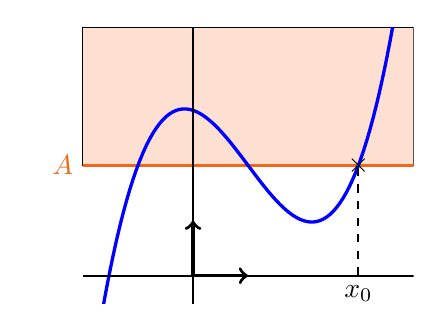
\begin{tikzpicture}[scale=0.7]
\clip (-3,-0.5) rectangle (4,4.5);
\draw [fill=ocre!20] (-2,2) -- (4,2) -- (4,4.5) -- (-2,4.5) -- cycle;

\draw [very thick, ocre, domain = -2:37] plot (\x,2);
\draw [blue, very thick,domain=-2:4,samples=100] plot (\x,{\x*\x*\x/3-\x*\x-\x/3+3});

\draw  [ocre](-2,2) node[left] {$A$};
\draw  (3,0) node[below] {$x_0$};
\draw [thick, dashed] (3,0) -- (3,2);
\draw (3,2) node {$\times$};
\draw [thick] (-2,0)--(4,0);
\draw [thick] (0,-2)--(0,5);
\draw [->, very thick] (0,0)--(1,0);
\draw [->,very thick] (0,0)--(0,1);


\end{tikzpicture}
\end{center}
\end{minipage}\end{example}





\begin{definition}On suppose qu'il existe un réel $a$ tel que $]-\infty ; a ] \subset D$.
\begin{itemize}
\item On dit que $f$ a pour limite $+\infty$ en $-\infty$ si, pour tout réel $A$, il existe un réel $x_0 \in D$ tel que, pour tout $x \in D$, si $x  \leqslant x_0$, alors $f(x) \geqslant A$. On notera $\displaystyle \lim_{x \to -\infty} f(x)=+\infty$.
\item On dit que $f$ a pour limite $-\infty$ en $-\infty$ si, pour tout réel $A$, il existe un réel $x_0 \in D$ tel que, pour tout $x \in D$, si $x  \leqslant x_0$, alors $f(x) \leqslant A$. On notera $\displaystyle \lim_{x \to -\infty} f(x)=-\infty$.\end{itemize}\end{definition}

\begin{example}
 On représente ici une fonction $f$ dans un repère.
 
\begin{minipage}{0.55\linewidth}
 Pour n'importe quel $A$, aussi grand que l'on veut, on peut trouver un $x_0$ en-dessous duquel la courbe est toujours au-dessus de la droite d'équation $y=A$. 

On a  $\displaystyle \lim_{x \to -\infty} f(x)=+\infty$ .

\end{minipage}\hfill\begin{minipage}{0.35\linewidth}
\begin{center}
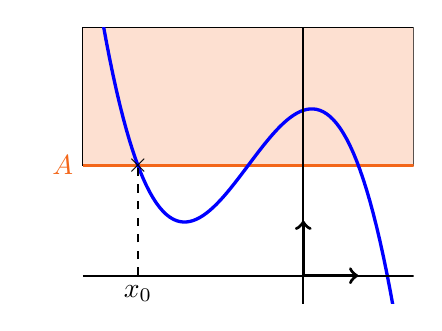
\begin{tikzpicture}[scale=0.7]
\clip (-5,-0.5) rectangle (2,4.5);
\draw [fill=ocre!20] (-4,2) -- (2,2) -- (2,4.5) -- (-4,4.5) -- cycle;

\draw [very thick, ocre, domain = -4:37] plot (\x,2);
\draw [blue, very thick,domain=-4:2,samples=100] plot (\x,{-\x*\x*\x/3-\x*\x+\x/3+3});

\draw  [ocre](-4,2) node[left] {$A$};
\draw  (-3,0) node[below] {$x_0$};
\draw [thick, dashed] (-3,0) -- (-3,2);
\draw (-3,2) node {$\times$};
\draw [thick] (-4,0)--(4,0);
\draw [thick] (0,-2)--(0,5);
\draw [->, very thick] (0,0)--(1,0);
\draw [->,very thick] (0,0)--(0,1);


\end{tikzpicture}
\end{center}
\end{minipage}
\end{example}


Il s'agit de la principale différence avec les suites : pour les suites, l'indice $n$ ne pouvait que tendre vers $+\infty$. Dans le cas des fonctions, le réel $x$ peut aller vers $+\infty$ mais aussi $-\infty$ et d'autres valeurs réelles entre les deux, comme nous le verrons plus tard dans ce chapitre...


\subsection{Limite finie en l'infini}

\begin{definition}On suppose qu'il existe un réel $a$ tel que $[a;+\infty [ \subset D$. Soit $l\in\mathbb{R}$.
\begin{itemize}
\item On dit que $f$ a pour limite $\ell$ en $+\infty$ (ou que $f(x)$ tend vers $\ell$ lorsque $x$ tend vers $+\infty$) si, pour tout $\varepsilon>0$, il existe un réel $x_0$ tel que, si $x \geqslant x_0$, alors $f(x) \in ]\ell-\varepsilon ; \ell+\varepsilon [$.\\ Si une telle limite existe, elle est unique. On note alors $\displaystyle \lim_{x \to +\infty} f(x)=\ell$.
\item On dit que $f$ a pour limite $\ell$ en $-\infty$ (ou que $f(x)$ tend vers $\ell$ lorsque $x$ tend vers $-\infty$) si, pour tout $\varepsilon>0$, il existe un réel $x_0$ tel que, si $x \leqslant x_0$, alors $f(x) \in ]\ell-\varepsilon ; \ell+\varepsilon [$.\\ Si une telle limite existe, elle est unique. On note alors $\displaystyle \lim_{x \to -\infty} f(x)=\ell$.
\end{itemize}\end{definition}

\begin{example} Une fonction $f$ est représentée ci-dessous. Pour n'importe quel $\varepsilon>0$, on peut trouver un réel $x_0$ à partir duquel on a toujours $f(x) \in ]2-\varepsilon ; 2+\varepsilon [$. On a  $\displaystyle \lim_{x \to +\infty} f(x)=2$.

\begin{center}

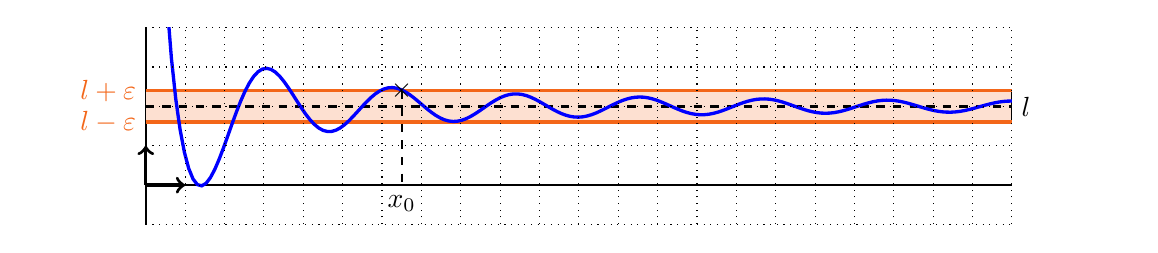
\begin{tikzpicture}[scale=0.5]
\clip (-3,-1) rectangle (25,4);
\draw [thick] (0,0)--(22,0);
\draw [thick] (0,-2)--(0,28);
\draw [->, very thick] (0,0)--(1,0);
\draw [->,very thick] (0,0)--(0,1);

\draw [fill=ocre!20] (0,1.6) -- (22,1.6) -- (22,2.4) -- (0,2.4) -- cycle;
\draw [very thick, ocre, domain = 0:22] plot (\x,1.6);
\draw [very thick, ocre, domain = 0:22] plot (\x,2.4);
\draw [very thick, dashed, domain = 0:22] plot (\x,2);
\draw [very thick, blue, domain = 0.1:22, samples =200] plot (\x,{2+3*cos(2*deg(\x))/\x}) ;
\draw [ thin, dotted] (0,-2) grid (22,28);
\draw  [thick] (6.5,2.4) node {$\times$};
\draw [thick, dashed] (6.5, 2.4) -- (6.5,0);
\draw  [thick] (6.5,0) node[below] {$x_0$};

\draw  [ocre](0,1.6) node[left] {$l-\varepsilon$};
\draw  [ocre](0,2.4) node[ left] {$l+\varepsilon$};
\draw  (22,2) node[right] {$l$};

\end{tikzpicture}
\end{center}\end{example}


\begin{definition} On se place dans un repère $(0;\vec i, \vec j)$ orthonormé.
\begin{itemize}
\item Si $\displaystyle \lim_{x \to +\infty} f(x)=\ell$, on dit que la droite d'équation $y=l$ est asymptote à la courbe de $f$ en $+\infty$
\item Si $\displaystyle \lim_{x \to -\infty} f(x)=\ell$, on dit que la droite d'équation $y=l$ est asymptote à la courbe de $f$ en $-\infty$\end{itemize} \end{definition}

\begin{example}Dans le cas précédent, la droite d'équation $y=2$ est asymptote à la courbe de $f$ en $+\infty$.\end{example}


Comme dans le cas des suites, il est parfois utile de préciser le comportement d'une fonction qui admet une limite finie en $+\infty$.

\begin{definition}On suppose qu'il existe un réel $a$ tel que $[a;+\infty [ \subset D$. Soit $l\in\mathbb{R}$.
\begin{itemize}
\item On dit que $f(x)$ tend vers $\ell$ par valeurs supérieures lorsque $x$ tend vers $+\infty$ si, pour tout $\varepsilon>0$, il existe un réel $x_0$ tel que, si $x \geqslant x_0$, alors $f(x) \in ]\ell ; \ell+\varepsilon [$. Autrement dit, la limite de $f$ en $+\infty$ vaut $\ell$ et $f(x)$ reste supérieur à $\ell$ à partir d'un certain réel. On note alors $\displaystyle \lim_{x \to +\infty} f(x)=\ell^+$.
\item On dit que $f(x)$ tend vers $\ell$ par valeurs inférieures lorsque $x$ tend vers $+\infty$ si, pour tout $\varepsilon>0$, il existe un réel $x_0$ tel que, si $x \geqslant x_0$, alors $f(x) \in ]\ell-\varepsilon ; \ell [$. Autrement dit, la limite de $f$ en $+\infty$ vaut $\ell$ et $f(x)$ reste inférieur à $\ell$ à partir d'un certain réel. On note alors $\displaystyle \lim_{x \to +\infty} f(x)=\ell^-$.
\end{itemize}\end{definition}

Attention, ce n'est pas parce que $\displaystyle \lim_{x \to +\infty} f(x)=\ell$ qu'on a forcément $\displaystyle \lim_{x \to +\infty} f(x)=\ell^+$ ou $\displaystyle \lim_{x \to +\infty} f(x)=\ell^-$. Les valeurs de $f(x)$ peuvent osciller autour de $\ell$, lui étant parfois supérieures, parfois inférieures.

Les mêmes définitions s'étendent naturellement pour les limites en $-\infty$.

\begin{example}On a représenté la courbe d'une fonction $f$ dans un repère.

\begin{minipage}{0.65\linewidth}
Il semblerait que $\displaystyle\lim_{x\to +\infty}f(x)=2^-$ et $\displaystyle\lim_{x\to -\infty}f(x)=(-1)^+$

La droite d'équation $y=2$ est asymptote à la courbe de $f$ en $+\infty$.

La droite d'équation $y=-1$ est asymptote à la courbe de $f$ en $-\infty$.
\end{minipage}\hfill \begin{minipage}{0.3\linewidth}
\begin{flushright}

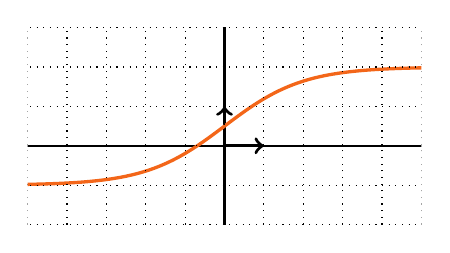
\begin{tikzpicture}[scale=0.5]
\clip (-5,-2) rectangle (5,3);
\draw [thick] (-10,0)--(22,0);
\draw [thick] (0,-2)--(0,28);
\draw [->, very thick] (0,0)--(1,0);
\draw [->,very thick] (0,0)--(0,1);

\draw [very thick, ocre, domain = -5:5, samples =200] plot (\x,{3/(1+exp(-\x))-1}) ;
\draw [thin, dotted] (-10,-2) grid (22,28);

\end{tikzpicture}
\end{flushright}\end{minipage}\end{example}


\subsection{Limites usuelles}

\begin{proposition}Soit $n$ un entier naturel non nul.
\[\displaystyle \lim_{x \to +\infty} x^n = +\infty \qquad \qquad \displaystyle \lim_{x \to +\infty} \dfrac{1}{x^n} = 0\]
\textbf{Si $n$ est pair}, \[\displaystyle \lim_{x \to -\infty} x^n = +\infty \qquad \qquad \displaystyle \lim_{x \to -\infty} \dfrac{1}{x^n}=0^+\]
\textbf{Si $n$ est impair}, 
\[\displaystyle \lim_{x \to -\infty} x^n = -\infty \qquad \qquad \displaystyle \lim_{x \to -\infty} \dfrac{1}{x^n}=0^-\]
Enfin, 
\[\displaystyle \lim_{x \to +\infty} \sqrt{x} = +\infty \qquad \qquad \displaystyle \lim_{x \to +\infty} \e^x = +\infty \qquad \qquad \displaystyle \lim_{x \to -\infty} \e^x = 0\]
\end{proposition}

Il est important de visualiser les courbes représentatives de ces fonctions. Celles-ci vous permettront de bien garder ces limites usuelles en tête.

\begin{minipage}{0.2\linewidth}
\begin{center}
\textbf{$x \mapsto x^n$, $n$ pair}
\end{center}
\begin{center}
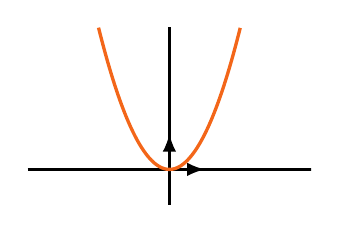
\begin{tikzpicture}[scale=0.45]
\clip (-4,-1) rectangle (4,4);
\draw [thick] (-4,0)--(7,0);
\draw [thick] (0,-4) -- (0,5);
\draw [very thick,->,>=latex] (0,0)--(0,1);
\draw [very thick,->,>=latex] (0,0)--(1,0);
\draw [very thick, ocre,domain=-2:2,samples=100] plot (\x,{\x*\x});
\end{tikzpicture}
\end{center}
\end{minipage}\hfill\begin{minipage}{0.2\linewidth}

\begin{center}
\textbf{$x \mapsto \frac{1}{x^n}$, $n$ pair}
\end{center}
\begin{center}
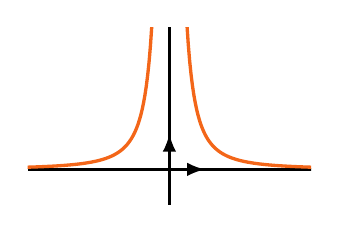
\begin{tikzpicture}[scale=0.45]
\clip (-4,-1) rectangle (4,4);
\draw [thick] (-4,0)--(7,0);
\draw [thick] (0,-4) -- (0,5);
\draw [very thick,->,>=latex] (0,0)--(0,1);
\draw [very thick,->,>=latex] (0,0)--(1,0);
\draw [very thick, ocre,domain=-4:-0.1,samples=100] plot (\x,{1/(\x*\x)});
\draw [very thick, ocre,domain=0.1:4,samples=100] plot (\x,{1/(\x*\x)});
\end{tikzpicture}
\end{center}
\end{minipage}\hfill
\begin{minipage}{0.2\linewidth}
\begin{center}
\textbf{$x \mapsto \e^x$}
\end{center}
\begin{center}
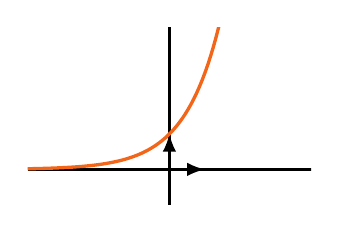
\begin{tikzpicture}[scale=0.45]
\clip (-4,-1) rectangle (4,4);
\draw [thick] (-4,0)--(7,0);
\draw [thick] (0,-4) -- (0,5);
\draw [very thick,->,>=latex] (0,0)--(0,1);
\draw [very thick,->,>=latex] (0,0)--(1,0);
\draw [very thick, ocre,domain=-4:4,samples=100] plot (\x,{exp(\x)});
\end{tikzpicture}
\end{center}\end{minipage}


\vskip10pt

\begin{minipage}{0.2\linewidth}
\begin{center}
\textbf{$x \mapsto x^n$, $n$ impair}
\end{center}
\begin{center}
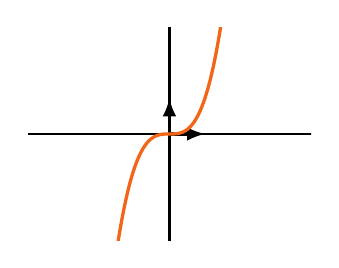
\begin{tikzpicture}[scale=0.45]
\clip (-4,-3) rectangle (4,3);
\draw [thick] (-4,0)--(7,0);
\draw [thick] (0,-4) -- (0,5);
\draw [very thick,->,>=latex] (0,0)--(0,1);
\draw [very thick,->,>=latex] (0,0)--(1,0);
\draw [very thick, ocre,domain=-2:2,samples=100] plot (\x,{\x*\x*\x});
\end{tikzpicture}
\end{center}
\end{minipage}\hfill\begin{minipage}{0.2\linewidth}
\begin{center}
\textbf{$x \mapsto \frac{1}{x^n}$, $n$ impair}
\end{center}
\begin{center}
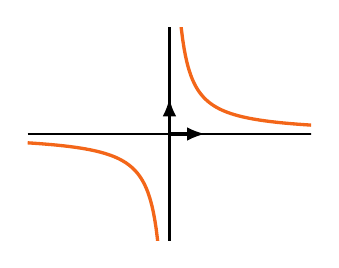
\begin{tikzpicture}[scale=0.45]
\clip (-4,-3) rectangle (4,3);
\draw [thick] (-4,0)--(7,0);
\draw [thick] (0,-4) -- (0,5);
\draw [very thick,->,>=latex] (0,0)--(0,1);
\draw [very thick,->,>=latex] (0,0)--(1,0);
\draw [very thick, ocre,domain=-4:-0.1,samples=100] plot (\x,{1/(\x)});
\draw [very thick, ocre,domain=0.1:4,samples=100] plot (\x,{1/(\x)});
\end{tikzpicture}
\end{center}
\end{minipage}\hfill\begin{minipage}{0.2\linewidth}
\begin{center}
\textbf{$x \mapsto \sqrt{x}$}
\end{center}
\begin{center}
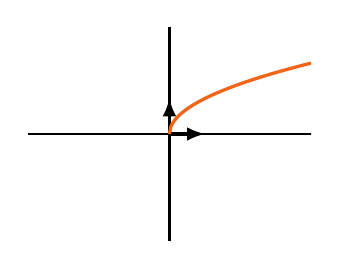
\begin{tikzpicture}[scale=0.45]
\clip (-4,-3) rectangle (4,3);
\draw [thick] (-4,0)--(7,0);
\draw [thick] (0,-4) -- (0,5);
\draw [very thick,->,>=latex] (0,0)--(0,1);
\draw [very thick,->,>=latex] (0,0)--(1,0);
\draw [very thick, ocre,domain=0:4,samples=100] plot (\x,{sqrt(\x)});
\end{tikzpicture}
\end{center}
\end{minipage}




\section{Limite en un point}

\subsection{Limite finie en un point}

\begin{definition}Soit $a \in D$ et $l$ un réel.

On dit que $f(x)$ tend vers $\ell$ lorsque $x$ tend vers $a$  si, pour tout $\varepsilon>0$, il existe un réel $\delta >0$ tel que, si $x\in ]a - \delta ; a+\delta[$, alors $f(x) \in ]\ell-\varepsilon : \ell+ \varepsilon [$.

Autrement dit, tout intervalle ouvert centré en $\ell$ contient toutes les valeurs de $x$ lorsque $x$ est suffisamment proche de $a$.

Si elle existe, une telle limite est unique. On note alors $\displaystyle \lim_{x \to a} f(x) =\ell $\end{definition}

Certaines fonctions admettent une limite finie différente si l'on se rapproche de $a$ par valeurs supérieurs ou par valeurs inférieures. Nous aurons l'occasion d'en discuter plus amplement dans le chapitre suivant.

\subsection{Limite infinie en un point}

\begin{definition}Soit $a \in D$ ou sur un bord de $D$.
\begin{itemize}
\item On dit que $f(x)$ tend vers $+\infty$ lorsque $x$ tend vers $a$  si, pour tout réel $A$, il existe un réel $\delta >0$ tel que, si $x\in ]a - \delta ; a+\delta[\cap D$, alors $f(x) > A$. Autrement dit, l'intervalle $]A;+\infty[$ contient toutes les valeurs de $f(x)$ lorsque $x$ est suffisamment proche de $a$. On note alors $\displaystyle \lim_{x \to a} f(x) =+\infty $.
\item On dit que $f(x)$ tend vers $-\infty$ lorsque $x$ tend vers $a$  si, pour tout réel $A$, il existe un réel $\delta >0$ tel que, si $x\in ]a - \delta ; a+\delta[\cap D$, alors $f(x) < A$. On note alors $\displaystyle \lim_{x \to a} f(x) =-\infty $.
\end{itemize}
\end{definition}

\begin{example} On a tracé ci-dessous la représentation graphique d'une fonction $f$.

\begin{center}

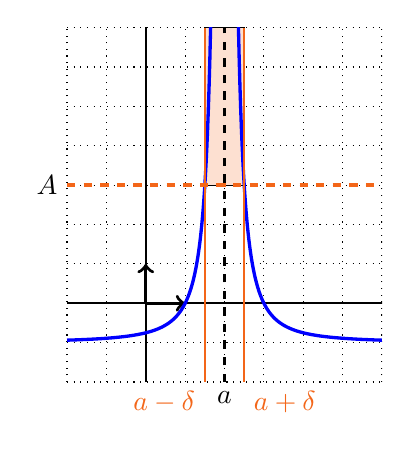
\begin{tikzpicture}[scale=0.5]
\clip (-3,-3) rectangle (6,7);
\draw [thick] (-2,0)--(22,0);
\draw [thick] (0,-2)--(0,28);
\draw [->, very thick] (0,0)--(1,0);
\draw [->,very thick] (0,0)--(0,1);
\draw [ thin, dotted] (-2,-2) grid (22,28);

\draw [fill=ocre!20] (1.5,3) -- (2.5,3) -- (2.5,7) -- (1.5,7) -- cycle;
\draw [very thick, blue, domain = -2:1.8, samples =200] plot (\x,{1/((\x-2)*(\x-2))-1}) ;
\draw [very thick, blue, domain = 2.2:6, samples =200] plot (\x,{1/((\x-2)*(\x-2))-1}) ;

\draw [very thick,ocre, dashed, domain = -2:22] plot (\x,3);

\draw [thick, ocre] (1.5,-2) -- (1.5,7);
\draw [thick, ocre] (2.5,-2) -- (2.5,7);
\draw [very thick, dashed] (2,-2) -- (2,7);

\draw  [ocre](1.5,-2) node[below left] {$a-\delta$};
\draw  [ocre](2.5,-2) node[below right] {$a+\delta$};
\draw  (2,-2) node[below] {$a$};
\draw  (-2,3) node[left] {$A$};

\end{tikzpicture}
\end{center}

Pour n'importe quelle valeur du réel $A$, on peut trouver un intervalle centré sur $a$ tel que toute valeur de $f(x)$ est supérieur à $A$ pour n'importe quel $x$ pris dans cet intervalle. Ce raisonnement vaut peu importe la valeur du réel $A$ : on a $\displaystyle \lim_{x \to a} f(x) =+\infty $.\end{example}


Tout comme précédemment, le comportement de la fonction $f$ peut varier selon si l'on approche du réel $a$ par valeurs inférieures ou supérieures. Il nous faut donc distinguer ces deux cas.

\newpage

\begin{definition}Soit $a \in D$ ou sur un bord de $D$.
\begin{itemize}
\item On dit que $f(x)$ tend vers $+\infty$ lorsque $x$ tend vers $a$ par valeurs inférieures  si, pour tout réel $A$, il existe un réel $\delta >0$ tel que, si $x\in ]a - \delta ; a[\cap D$, alors $f(x) > A$. Autrement dit, l'intervalle $]A;+\infty[$ contient toutes les valeurs de $f(x)$ lorsque $x$ est suffisamment proche de $a$ tout en lui étant inférieur. On note alors $\displaystyle \lim_{x \to a^-} f(x) =+\infty $.
\item On dit que $f(x)$ tend vers $+\infty$ lorsque $x$ tend vers $a$ par valeurs supérieures  si, pour tout réel $A$, il existe un réel $\delta >0$ tel que, si $x\in ]a ; a+\delta[\cap D$, alors $f(x) > A$. Autrement dit, l'intervalle $]A;+\infty[$ contient toutes les valeurs de $f(x)$ lorsque $x$ est suffisamment proche de $a$ tout en lui étant supérieur. On note alors $\displaystyle \lim_{x \to a^+} f(x) =+\infty $.
\end{itemize}
\end{definition}

Là encore, ces définitions peuvent s'étendre pour une limite valant $-\infty$.


\begin{example} On considère la fonction $f:x\mapsto \dfrac{1}{x-1}$, définie sur $\mathbb{R} \setminus \{1\}$, dont on a tracé ci-dessous la courbe dans un repère.

\begin{minipage}{0.3\linewidth}
\begin{center}

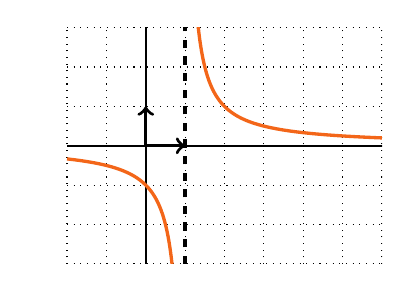
\begin{tikzpicture}[scale=0.5]
\clip (-3,-3) rectangle (6,3);
\draw [thick] (-2,0)--(22,0);
\draw [thick] (0,-3)--(0,28);
\draw [->, very thick] (0,0)--(1,0);
\draw [->,very thick] (0,0)--(0,1);
\draw [ thin, dotted] (-2,-3) grid (22,28);

\draw [very thick, ocre, domain = -2:0.8, samples =200] plot (\x,{1/(\x-1)}) ;
\draw [very thick, ocre, domain = 1.2:6, samples =200] plot (\x,{1/((\x-1)}) ;

\draw [very thick, dashed] (1,-3) -- (1,7);


\end{tikzpicture}
\end{center}
\end{minipage}\hfill\begin{minipage}{0.65\linewidth}

Il semblerait que, lorsque l'on s'approche de $1$ par valeurs supérieures, la limite soit $+\infty$, ce que l'on notera $\displaystyle \lim_{x \to 1^+} f(x) =+\infty $.
\vskip5pt
En revanche, lorsque l'on s'approche de $1$ par valeurs inférieures, la limite semble être $-\infty$, ce que l'on note $\displaystyle \lim_{x \to 1^-} f(x) =-\infty $. \end{minipage}
\end{example}



\begin{definition}Lorsque la limite d'une fonction $f$ est infinie en un point $a$, on dit que la droite d'équation $x=a$ est une asymptote verticale à la courbe représentative de $f$.\end{definition}

\begin{example} Dans l'exemple précédent, la droite d'équation $x=1$ est asymptote à la courbe de $f$.\end{example}


\section{Opérations sur les limites}

Les opérations sur les limites sont similaires à celles connues sur les suites. Dans cette partie, $f$ et $g$ sont deux fonctions définies au voisinages de $a$, $a$ pouvant être un réel, $+\infty$ ou $-\infty$. $l_1$ et $l_2$ sont deux réels.

\subsection{Limite de la somme}

\begin{proposition}[Limite de la somme] On a :

\begin{center}
\begin{tabularx}{\linewidth}{|l|X|X|X|X|X|X|}
\hline
$\displaystyle \lim_{x \to a} f(x)$ & $l_1$ & $l_1$ & $l_1$ & $+\infty$ & $-\infty$ & $ +\infty$\\
\hline
$\displaystyle \lim_{x \to a} g(x)$ & $l_2$ & $+\infty$ & $-\infty$ & $+\infty$ & $-\infty$ & $-\infty$ \\
\hline
$\displaystyle \lim_{x \to a} (f(x)+g(x))$ & $l_1+l_2$ & $+\infty$ & $-\infty$ & $+\infty$ & $-\infty$  & \textbf{FI}\\
\hline
\end{tabularx}
\end{center}\end{proposition}

\newpage


\subsection{Limite du produit}


\begin{proposition}[Limite du produit].
\begin{center}

\begin{tabularx}{\linewidth}{|l|X|X|X|X|}
\hline
$\displaystyle \lim_{x \to a} f(x)$ & $l_1 $ & $l_1 \neq 0$ & $\infty$ & $0$ \\
\hline
$\displaystyle \lim_{x \to a} g(x)$ & $l_2$ & $\infty$ &  $\infty$ & $\infty$ \\
\hline
$\displaystyle \lim_{x \to a} (f(x)\,g(x))$ & $l_1\,l_2$ & $\infty$ (r.s.) & $\infty$ (r.s)& \textbf{FI} \\
\hline
\end{tabularx}

 \textbf{r.s. : Règle des signes}
 \end{center} \vspace{-1cm}
\end{proposition}

\begin{example}On considère la fonction $f$ définie pour tout réel $x$ non nul par $f(x)=x^2-x+\dfrac{1}{x}$.

D'une part, $\displaystyle\lim_{x \to -\infty} x^2 = +\infty$, $\displaystyle\lim_{x \to -\infty} (-x) = +\infty$ et $\displaystyle\lim_{x \to -\infty} \dfrac{1}{x} = 0$. Ainsi, par somme, $\displaystyle\lim_{x \to -\infty} f(x) = +\infty$.

Toutefois, si l'on étudie la limite en $+\infty$, nous aboutissons à une forme indéterminée « $\infty - \infty$ ». Il est alors possible d'utiliser les techniques de calcul déjà employées lors du chapitre sur l'étude des limites de suite, en particulier la factorisation par le terme de plus haut degré. 

Ainsi, pour tout réel non nul $x$, $f(x)=x^2 \times \left(1-\dfrac{1}{x}+\dfrac{1}{x^3}\right)$.

Or, $\displaystyle\lim_{x \to +\infty}x^2=+\infty$ et $\displaystyle\lim_{x \to +\infty}\left(1-\dfrac{1}{x}+\dfrac{1}{x^3}\right)=1$. Ainsi, par produits, $\displaystyle\lim_{x \to +\infty}f(x)=+\infty$.\end{example}

\subsection{Limite du quotient}

\begin{proposition}[Limite du quotient] Dans cette partie, on suppose $l_2 \neq 0$.
\begin{center}

\begin{tabularx}{\linewidth}{|l|X|X|X|X|X|X|}
\hline
$\displaystyle \lim_{x \to a} f(x)$ & $l_1 $ & $l_1$ & $l_1 \neq 0$ & $\infty$ & 0 & $\infty$ \\
\hline
$\displaystyle \lim_{x \to a} g(x)$ & $l_2$ & $\infty$ &  $0^+$ ou $0^-$ & $l_2$, $0^+$ ou $0^-$  & $0$ & $\infty$ \\
\hline
$\displaystyle \lim_{x \to a} \left(\dfrac{f(x)}{g(x)}\right)$ & $\dfrac{l_1}{l_2}$ & 0 & $\infty$ (r.s.) & $\infty$ (r.s.) & \textbf{FI} & \textbf{FI} \\
\hline
\end{tabularx}

 \textbf{r.s. : Règle des signes}
 \end{center} \vspace{-1cm}
\end{proposition}

\begin{example}Pour tout réel $x$, on pose $f(x)=\dfrac{1-2x^4}{1+x^2}$. L'étude des limites en $+\infty$ et $-\infty$ de $f$ aboutit à une forme indéterminée. Or, pour tout réel non nul $x$,
\[f(x)= \dfrac{x^4}{x^2} \times \dfrac{\frac{1}{x^4}-2}{\frac{1}{x^2}+1} = x^2 \times \dfrac{\frac{1}{x^4}-2}{\frac{1}{x^2}+1}.\]
Or, $\displaystyle\lim_{x \to +\infty}x^2=+\infty$, $\displaystyle\lim_{x \to +\infty}\left(\frac{1}{x^4}-2\right)=-2$ et $\displaystyle\lim_{x \to +\infty}\left(\frac{1}{x^2}+1\right)=1$. Ainsi, en appliquant les règles de calcul sur les produits et quotients de limite, on aboutit à $\displaystyle\lim_{x \to +\infty}f(x)=-\infty$.\end{example}

\begin{example}On considère la fonction $f$ définie pour tout réel $x\neq 2$ par $f(x)=\dfrac{3x+1}{2x-4}$.

Pour tout réel $x\neq 2$ et $x\neq 0$, on a alors $f(x)=\dfrac{x\left(3+\dfrac{1}{x}\right)}{x\left(2-\dfrac{4}{x}\right)}=\dfrac{3+\dfrac{1}{x}}{2-\dfrac{4}{x}}$.

Or, $\displaystyle \lim_{x \to +\infty} \left(\dfrac{1}{x}\right) = 0$ et $\displaystyle \lim_{x \to +\infty} \left(\dfrac{4}{x}\right) = 0$.

Ainsi, $\displaystyle \lim_{x \to +\infty} f(x)=\dfrac{3}{2}$. De la même manière, on montre que $\displaystyle \lim_{x \to -\infty} f(x)=\dfrac{3}{2}$\end{example}


\begin{example} On considère la fonction $f:x\mapsto \sqrt{x} + \dfrac{1}{1-x}$, définie sur $[0;1[ \cup ]1;+\infty[$.

\textbf{Pour calculer la limite en $1^+$ :}
\begin{itemize}
\item $\displaystyle \lim_{x \to 1^+} \sqrt{x} = \sqrt{1}=1$.
\item $\displaystyle \lim_{x \to 1} (1-x)=1-1=0$. Par ailleurs, si $x \geqslant 1$, alors $1-x \leqslant 0$ et donc $\displaystyle \lim_{x \to 1^+} (1-x)=0^-$. 

Ainsi, par quotient de limites, $\displaystyle \lim_{x \to 1^+} \dfrac{1}{1-x}=-\infty$.
\item Par somme de limites, $\displaystyle \lim_{x \to 1^+} f(x)=-\infty$.

\end{itemize}


\textbf{Pour calculer la limite en $1^-$ :}
\begin{itemize}
\item $\displaystyle \lim_{x \to 1^-} \sqrt{x} = \sqrt{1}=1$.
\item $\displaystyle \lim_{x \to 1} (x-1)=1-1=0$. Par ailleurs, si $x \leqslant 1$, alors $1-x \geqslant 0$ et donc $\displaystyle \lim_{x \to 1^-} (1-x)=0^+$. 

Ainsi, par quotient de limites, $\displaystyle \lim_{x \to 1^+} \dfrac{1}{1-x}=+\infty$.
\item Par somme de limites, $\displaystyle \lim_{x \to 1^-} f(x)=+\infty$.
\end{itemize}

\textbf{Pour calculer la limite en $+\infty$ :}
\begin{itemize}
\item $\displaystyle \lim_{x \to +\infty} \sqrt{x} =+\infty$. 
\item $\displaystyle \lim_{x \to +\infty} (1-x)=-\infty$, ainsi, par quotient de limites, $\displaystyle \lim_{x \to +\infty} \dfrac{1}{1-x}=0$.
\item Par somme de limites, $\displaystyle \lim_{x \to +\infty} f(x)=+\infty$.
\end{itemize}

Représenter la courbe de la fonction $f$ dans un graphique (par exemple, dans un logiciel de géométrie ou sur une calculatrice) permet de confirmer ou d'infirmer les calculs.


\begin{center}
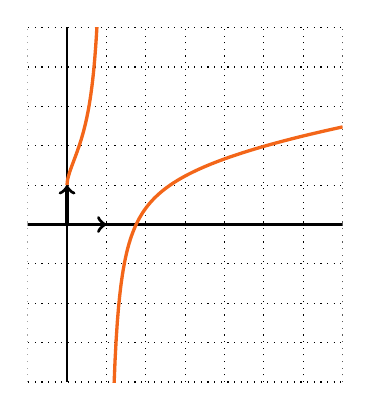
\begin{tikzpicture}[scale=0.5]
\clip (-1,-4) rectangle (7,5);
\draw [thick] (-2,0)--(22,0);
\draw [thick] (0,-4)--(0,28);
\draw [->, very thick] (0,0)--(1,0);
\draw [->,very thick] (0,0)--(0,1);
\draw [ thin, dotted] (-2,-4) grid (22,28);

\draw [very thick, ocre, domain = 0:0.9, samples =200] plot (\x,{sqrt(\x)+1/(1-\x)}) ;
\draw [very thick, ocre, domain = 1.1:7, samples =200] plot (\x,{{sqrt(\x)+1/(1-\x)}}) ;


\end{tikzpicture}
\end{center}
\vspace{-1cm}
\end{example}

\subsection{Composition de limites}

\begin{proposition}Soit $a$, $b$ et $c$ des réels ou $\pm \infty$. Soit $f$ et $g$ des fonctions définies sur $\mathbb{R}$.
On suppose que $\displaystyle\lim_{x \to a}f(x)=b$ et $\displaystyle\lim_{X \to b}g(X)=c$. Alors $\displaystyle\lim_{x \to a}(g \circ f)(x)=c$.
\end{proposition}


\begin{example} On considère la fonction $f:x\mapsto \e^{-2x^2-3x-5}$. 

On sait que $\displaystyle \lim_{x \to +\infty} (-2x^2-3x-5) = \color{red}{-\infty}$. Par ailleurs, $\displaystyle\lim_{X \to \color{red}{-\infty}}\color{black}\e^X=0$. 

Ainsi, par composition de limites, $\displaystyle \lim_{x \to +\infty} \e^{-2x^2-3x-5}=0$.\end{example}



\section{Comparaison de limites}

\begin{theorem}[Théorème de comparaison]Soit $a$ un réel ou $\pm \infty$. Soit $f$ et $g$ deux fonctions définies sur un intervalle $I$ dont $a$ est un élément ou un bord.
\begin{itemize}
\item Si, pour tout $x\in I$, $f(x)\geqslant g(x)$ et $\displaystyle \lim_{x \to a} g(x)=+\infty$, alors $\displaystyle \lim_{x \to a} f(x)=+\infty$.
\item Si, pour tout $x\in I$, $f(x)\leqslant g(x)$ et $\displaystyle \lim_{x \to a} g(x)=-\infty$, alors $\displaystyle \lim_{x \to a} f(x)=-\infty$.
\end{itemize}\end{theorem}

\begin{example}Pour tout réel $x$, on pose $f(x)=(2+\cos(x))\e^x$. 

Pour tout réel $x$, $\cos(x)\geqslant -1$, ce qui implique que $2+\cos(x)\geqslant 1$ d'où $f(x)\geqslant \e^x$. Or, $\displaystyle \lim_{x \to +\infty} \e^x=+\infty$. 

Ainsi, par comparaison, $\displaystyle \lim_{x \to +\infty} f(x)=+\infty$.\end{example}

\begin{example}On souhaite montrer que, justement, $\displaystyle \lim_{x \to +\infty}\e^x=+\infty$. 

Pour tout réel $x$, on pose $f(x)=\e^x-x$. $f$ est dérivable sur $\mathbb{R}$ et, pour tout réel $x$, $f'(x)=\e^x-1$. Ainsi, $f'(x)\leqslant 0 \Leftrightarrow x \leqslant 0$. On construit alors le tableau de signes de $f'$ et le tableau de variations de $f$.
\begin{center}
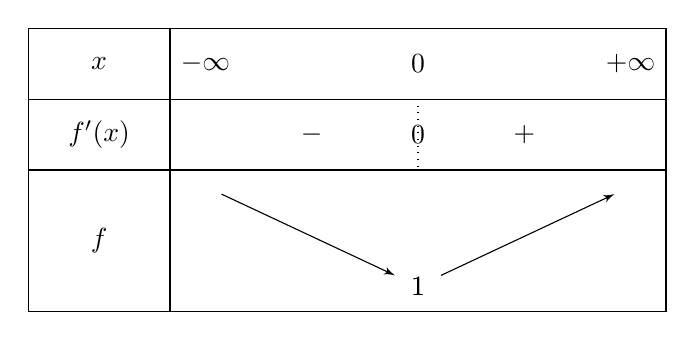
\begin{tikzpicture}[scale=0.9]
\tikzset{node style/.style = {inner sep = 2pt, outer sep = 2pt}}
   \tkzTabInit{$x$ / 1 , $f'(x)$ / 1, $f$ / 2}{$-\infty$, $0$, $+\infty$}
   \tkzTabLine{, -, z, +,  }
   \tkzTabVar{+/$ $,-/$1$,+/$ $}
\end{tikzpicture}
\end{center}

On s'aperçoit alors que, pour tout réel $x$, $f(x) \geqslant 1$, et donc que $\e^x \geqslant 1+x$. Or,  $\displaystyle \lim_{x \to +\infty} (1+x)=+\infty$. D'après le théorème de comparaison, on a donc que  $\displaystyle \lim_{x \to +\infty} \e^x = +\infty$.\end{example}

\newpage


\begin{theorem}[Théorème d'encadrement]Soit $a$ un réel. Soit $f$, $g$ et $h$ trois fonctions définies sur un intervalle $I$ dont $a$ est un élément ou un bord.

Si, pour tout $x\in I$, $f(x)\leqslant g(x)\leqslant$ et si $f$ et $h$ admettent une même limite \textbf{finie} $l$ en $a$, alors $g$ admet également une limite finie en $a$ et $\displaystyle \lim_{x \to +\infty} g(x)=l$.
\end{theorem}

\begin{example}Pour tout réel non nul $x$, on pose $f(x)=\dfrac{\cos(x)}{x}$. On a alors, pour tout $x>0$, $-\dfrac{1}{x} \leqslant f(x) \leqslant \dfrac{1}{x}$.

 Or, $\displaystyle \lim_{x \to +\infty} \left( \dfrac{1}{x}\right) =\displaystyle \lim_{x \to +\infty} \left(-\dfrac{1}{x}\right)=0$. 
 
 Ainsi, d'après le théorème d'encadrement, $\displaystyle \lim_{x \to +\infty}f(x)=0$.\end{example}
 
\begin{example}Pour tout réel non nul $x$, on pose $g(x)=x\,\sin\left(\dfrac{1}{x}\right)$.

Pour tout réel $x>0$, $-1\leqslant \sin\left(\dfrac{1}{x}\right)\leqslant 1$ et donc $-x \leqslant f(x) \leqslant x$. Or, $\displaystyle\lim_{x \to 0^+}(-x)=\displaystyle\lim_{x \to 0^+}x=0$. 

Ainsi, d'après le théorème d'encadrement, $\displaystyle\lim_{x \to 0^+}f(x)=0$.\end{example}


\section{Croissances comparées}

\begin{proposition}[Croissances comparées -- fonction exponentielle] Soit $n$ un entier naturel.
\[\displaystyle \lim_{x \to +\infty} \dfrac{\e^x}{x^n}=+\infty \qquad \qquad \displaystyle \lim_{x \to -\infty} x^n\,\e^x =0\]\end{proposition}


\begin{example} Pour tout réel $x$, on pose $f(x)=\dfrac{\e^x-x}{\e^x}$. On a alors $f(x)=\dfrac{\e^x}{\e^x}-\dfrac{x}{\e^x}=1-\dfrac{x}{\e^x}$.

Or, puisque $\displaystyle \lim_{x \to +\infty} \dfrac{\e^x}{x}=+\infty$, on a alors $\displaystyle \lim_{x \to +\infty} \dfrac{x}{\e^x}=0$. Ainsi, $\displaystyle \lim_{x \to +\infty} f(x)=1$.\end{example}

Cette proposition peut être vue comme la limite de nouvelles fonctions, les fonctions $x\mapsto \dfrac{\e^x}{x^n}$ et $x\mapsto x^n\,\e^x$. Il est alors possible d'utiliser tous les résultats précédents, en particuliers ceux sur la composition. Par exemple, si l'on considère une fonction $u$ telle que $\displaystyle\lim_{x \to a}u(x)=+\infty$, alors on aura $\displaystyle\lim_{x \to a}\dfrac{\e^{u(x)}}{u(x)}=+\infty$.

\textbf{Il est important de bien avoir la même expression dans l'exponentielle et au dénominateur !}

\begin{example}On considère la fonction $f : x\mapsto \dfrac{\e^{-2x+4}}{3x^3}$, définie sur $\mathbb{R}^*$. On souhaite déterminer $\displaystyle\lim_{x \to -\infty}f(x)$. Pour cela, il semble naturel de faire intervenir une croissance comparée. Seulement, les expressions dans l'exponentielle et au dénominateur sont différentes, il faut donc transformer légèrement cette écriture pour se ramener aux fonctions mentionnées dans la propriété.

Pour tout réel non nul $x$, 
\[\dfrac{\e^{-2x+4}}{3x^3} = \dfrac{\e^{-2x} \times \e^{4}}{3 \times x^3}=\dfrac{\e^4}{3} \times \dfrac{\e^{-2x}}{x^3}=\dfrac{\e^4}{3} \times \dfrac{(-2)^3 \times \e^{-2x}}{(-2)^3 \times x^3} = \dfrac{-8\e^4}{3} \times \dfrac{\e^{-2x}}{(-2x)^3}.\]

Or, $\displaystyle\lim_{x \to - \infty}(2x)=+\infty$, et, par croissances comparées, $\displaystyle \lim_{x \to +\infty} \dfrac{\e^X}{X^n}=+\infty$. 

Ainsi, par composition, $\displaystyle \lim_{x \to -\infty} \dfrac{\e^{-2x}}{(-2x)^3}=+\infty$. Enfin, par produit, $\displaystyle \lim_{x \to -\infty}=-\infty$.\end{example}



\section{Approfondissement : Asymptotes obliques}

\begin{definition}Soit $a$ un réel et $f$ une fonction définie sur $]a;+\infty[$. Soit $m$ et $p$ des réels. 

On dit que la droite d'équation $y=mx+p$ est asymptote à la courbe représentative de $f$ en $+\infty$ si \[\displaystyle \lim_{x \to +\infty} (f(x)-(mx+p))=0.\]\end{definition}


\begin{example} On considère la fonction $f:x\mapsto \dfrac{x^2+3x-3}{2x-2}$, définie sur $\mathbb{R}\setminus \{1\}$. Pour tout $x\neq 1$, 
\[f(x)-\left(\dfrac{1}{2}x+2\right)=\dfrac{x^2+3x-3}{2x-2}-\dfrac{\left(\dfrac{1}{2}x+2\right)(2x-2)}{2x-2}=\dfrac{x^2+3x-3-x^2-4x+x+4}{2x-2}=\dfrac{1}{2x-2}.\]

Ainsi, $\displaystyle \lim_{x \to +\infty} \left(f(x)-\left(\dfrac{1}{2}x+2\right)\right)=0$ et $\displaystyle \lim_{x \to -\infty} \left(f(x)-\left(\dfrac{1}{2}x+2\right)\right)=0$. 

La droite d'équation $y=\dfrac{1}{2}x+2$ est asymptote à la courbe représentative de $f$ en $+\infty$ et en $-\infty$.

Il est également possible, en étudiant le signe de $f(x)-\left(\dfrac{1}{2}x+2\right)$, de déterminer la position relative de la courbe de $f$ par rapport à son asymptote.
Ainsi, 
\[ f(x)-\left(\dfrac{1}{2}x+2\right) \leqslant 0 \Leftrightarrow \dfrac{1}{2x-2} \leqslant 0 \Leftrightarrow 2x-2 \leqslant 0 \Leftrightarrow x\leqslant 1.\]

La courbe de $f$ est en-dessous de son asymptote en $-\infty$ et est au-dessus en $+\infty$.

\begin{center}
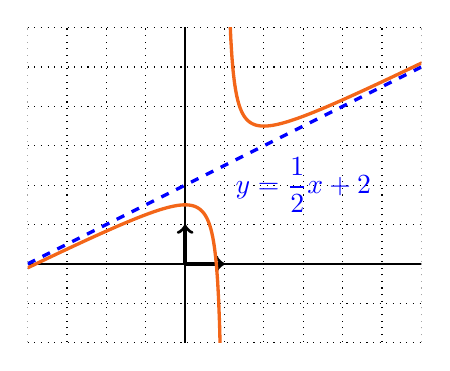
\begin{tikzpicture}[scale=0.5]
\clip (-4,-2) rectangle (6,6);
\draw [thick] (-4,0)--(22,0);
\draw [thick] (0,-4)--(0,28);
\draw [->, very thick] (0,0)--(1,0);
\draw [->,very thick] (0,0)--(0,1);
\draw [ thin, dotted] (-4,-4) grid (22,28);

\draw [very thick, ocre, domain = -4:0.9, samples =200] plot (\x,{(\x*\x+3*\x-3)/(2*\x-2)}) ;
\draw [very thick, ocre, domain = 1.1:7, samples =200] plot (\x,{(\x*\x+3*\x-3)/(2*\x-2)}) ;
\draw [very thick, blue, dashed, domain = -4:7, samples =200] plot (\x,{\x/2+2}) ;
\draw [blue] (3,2) node {$y=\dfrac{1}{2}x+2$};

\end{tikzpicture}
\end{center}
\vspace{-1cm}\end{example}

\chapter{Exercices}

\section*{Notion de limite}

\begin{exercise}[topic=lim21]On a représenté ci-dessous la courbe représentative $\mathcal{C}_f$ d'une fonction $f$ dans un repère orthonormé.

\begin{minipage}{0.5\linewidth}
\begin{center}
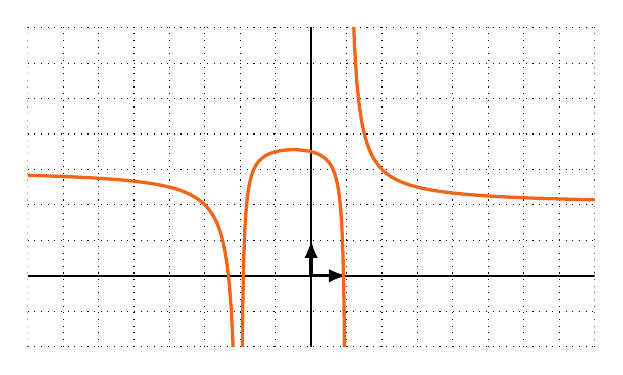
\begin{tikzpicture}[scale=0.45]
\clip (-8,-2) rectangle (8,7);
\draw [thin, dotted] (-8,-8) grid (8,8);
\draw [thick] (-8,0)--(8,0);
\draw [thick] (0,-8) -- (0,8);
\draw [very thick,->,>=latex] (0,0)--(0,1);
\draw [very thick,->,>=latex] (0,0)--(1,0);
\draw [very thick, ocre,domain=-1.99:0.99,samples=100] plot (\x,{(1/((\x+2)*(\x-1))+4});
\draw [very thick, ocre,domain=-8:-2.01,samples=100] plot (\x,{{(1/(\x+2)+3}});
\draw [very thick, ocre,domain=1.01:8,samples=100] plot (\x,{{(1/(\x-1)+2}});
\end{tikzpicture}
\end{center}
\end{minipage} \hfill \begin{minipage}{0.49\linewidth}
A l'aide de cette représentation graphique, déterminer $\displaystyle \lim_{x \to 1^+} f(x)$, $\displaystyle \lim_{x \to 1^-} f(x)$, $\displaystyle \lim_{x \to (-2)^+} f(x)$, $\displaystyle \lim_{x \to (-2)^-} f(x)$, $\displaystyle \lim_{x \to +\infty} f(x)$ et $\displaystyle \lim_{x \to -\infty} f(x)$.

\vskip10pt

Quelles sont les asymptotes verticales ou horizontales à la courbe représentative de la fonction $f$ ?
\end{minipage}

\end{exercise}

\begin{solution}D'après cette représentation graphique,
 $\displaystyle \lim_{x \to 1^+} f(x)=+\infty$,
$\displaystyle \lim_{x \to 1^-} f(x)=-\infty$, 
 $\displaystyle \lim_{x \to (-2)^+} f(x)=-\infty$,\\  $\displaystyle \lim_{x \to (-2)^-} f(x)=-\infty$,  $\displaystyle \lim_{x \to +\infty} f(x)=2$,
$\displaystyle \lim_{x \to -\infty} f(x)=3$.


De plus,
\begin{itemize}
\item La droite d'équation $x=1$ est asymptote verticale à la courbe de $f$.
\item La droite d'équation $x=-2$ est asymptote verticale à la courbe de $f$.
\item La droite d'équation $y=2$ est asymptote horizontale à la courbe de $f$ en $+\infty$.
\item La droite d'équation $y=3$ est asymptote horizontale à la courbe de $f$ en $-\infty$.
\end{itemize}\end{solution}





\begin{exercise}[topic=lim21]On considère une fonction $f$ dont la courbe représentative $\mathcal{C}_f$ est donnée ci-dessous.

\begin{minipage}{0.45\linewidth}
\begin{center}
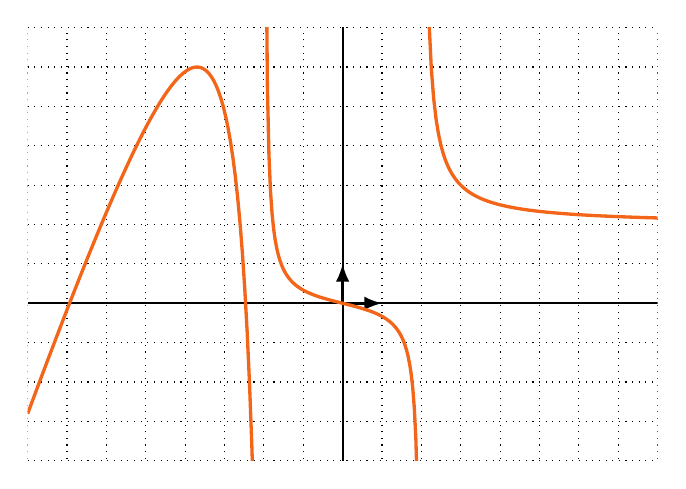
\begin{tikzpicture}[scale=0.5]
\clip (-8,-4) rectangle (8,7);
\draw [thin, dotted] (-8,-8) grid (8,8);
\draw [thick] (-8,0)--(8,0);
\draw [thick] (0,-8) -- (0,8);
\draw [very thick,->,>=latex] (0,0)--(0,1);
\draw [very thick,->,>=latex] (0,0)--(1,0);
\draw [very thick, ocre,domain=-8:-2,samples=100] plot (\x,{(3*(\x-0.3)*(\x-0.3)/((\x+1.7))+30});
\draw [very thick, ocre,domain=-1.99:1.9,samples=100] plot (\x,{\x/((\x-2)*(\x+2))});
\draw [very thick, ocre,domain=2.01:8,samples=100] plot (\x,{1/((\x-2))+2});
\end{tikzpicture}
\end{center}\end{minipage} \hfill \begin{minipage}{0.49\linewidth}

Déterminer graphiquement les valeurs de  $\displaystyle \lim_{x \to -\infty} f(x)$, $\displaystyle \lim_{x \to (-2)^-} f(x)$, $\displaystyle \lim_{x \to (-2)^+} f(x)$, $\displaystyle \lim_{x \to 2^-} f(x)$, $\displaystyle \lim_{x \to 2^+} f(x)$ et $\displaystyle \lim_{x \to +\infty} f(x)$.
\vskip10pt
Quelles sont les asymptotes horizontales et verticales à la courbe $\mathcal{C}_f$ ?\end{minipage} \end{exercise}

\begin{solution}
  $\displaystyle \lim_{x \to -\infty} f(x)=-\infty$, 
 $\displaystyle \lim_{x \to (-2)^-} f(x)=-\infty$,
 $\displaystyle \lim_{x \to (-2)^+} f(x)=+\infty$,
  $\displaystyle \lim_{x \to 2^-} f(x)=-\infty$,
 $\displaystyle \lim_{x \to 2^+} f(x)=+\infty$,
 $\displaystyle \lim_{x \to +\infty} f(x)=2$.

Par ailleurs,
\begin{itemize}
\item La droite d'équation $x=2$ est une asymptote verticale à la courbe de $f$.
\item La droite d'équation $x=-2$ est asymptote verticale à la courbe de $f$.
\item La droite d'équation $y=2$ est asymptote horizontale à la courbe de $f$ en $+\infty$.
\end{itemize}\end{solution}






\begin{exercise}[topic=lim21]On considère une fonction $f$ dont le tableau de variations est donnée ci-dessous. On note $\mathcal{C}_f$ la courbe représentative de $f$ dans un repère orthonormé.

\begin{center}
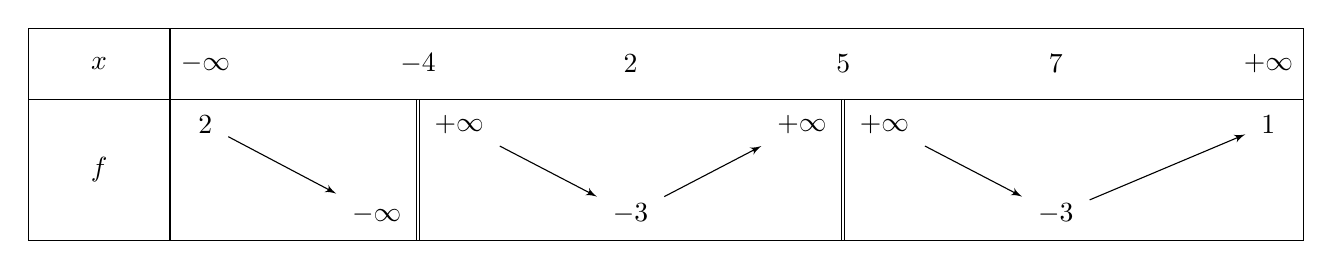
\begin{tikzpicture}[scale=0.9]
   \tkzTabInit{$x$ / 1 , $f$ / 2}{$-\infty$, $-4$,$2$,$5$,$7$, $+\infty$}
   \tkzTabVar{+/$2$,-D+/$-\infty$/$+\infty$,-/$-3$, +D+/ $+\infty$ / $+\infty$, -/$-3$, +/$1$ }
\end{tikzpicture}
\end{center}

\begin{enumerate}
\item Déterminer $\displaystyle \lim_{x \to -\infty} f(x)$, $\displaystyle \lim_{x \to (-4)^-} f(x)$, $\displaystyle \lim_{x \to (-4)^+} f(x)$, $\displaystyle \lim_{x \to 5^-} f(x)$, $\displaystyle \lim_{x \to 5^+} f(x)$ et $\displaystyle \lim_{x \to +\infty} f(x)$
\item Quelles sont les asymptotes horizontales et verticales à $\mathcal{C}_f$ ?
\item Dans un repère orthonormé, tracer une courbe d'une fonction compatible avec ce tableau de variations.
\end{enumerate}\end{exercise}

\begin{solution}
 $\displaystyle \lim_{x \to -\infty} f(x)=2$, 
 $\displaystyle \lim_{x \to (-4)^-} f(x)=-\infty$,  $\displaystyle \lim_{x \to (-4)^+} f(x)=+\infty$,  $\displaystyle \lim_{x \to 5^-} f(x)=+\infty$, 
 $\displaystyle \lim_{x \to 5^+} f(x)=+\infty$,
$\displaystyle \lim_{x \to +\infty} f(x)=1$.

Les droites d'équation $x=-4$ et $x=5$ sont asymptotes verticales à la courbe de $f$. La droite d'équation $y=2$ en est une asymptote horizontale en $-\infty$ et la droite d'équation $y=1$ l'est en $+\infty$.


\begin{center}
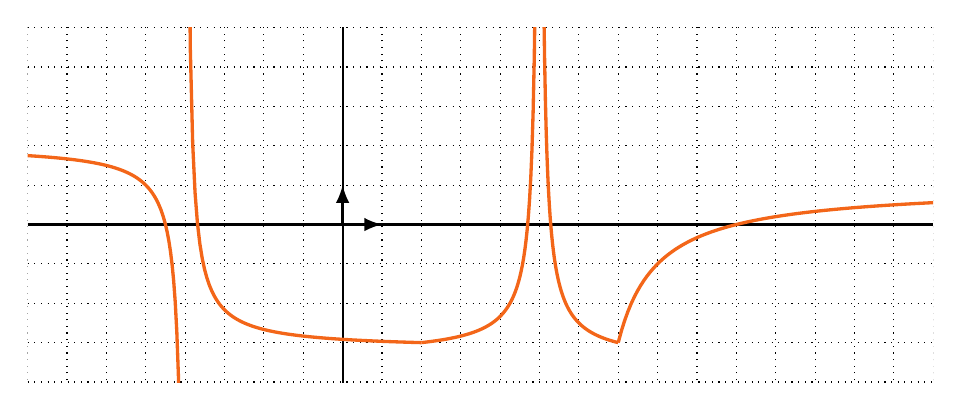
\begin{tikzpicture}[scale=0.5]
\clip (-8,-4) rectangle (15,5);
\draw [thin, dotted] (-8,-8) grid (15,8);
\draw [thick] (-8,0)--(15,0);
\draw [thick] (0,-8) -- (0,8);
\draw [very thick,->,>=latex] (0,0)--(0,1);
\draw [very thick,->,>=latex] (0,0)--(1,0);
\draw [very thick, ocre,domain=-8:-4.01,samples=100] plot (\x,{(1/(\x+4)+2});
\draw [very thick, ocre,domain=-3.99:2,samples=100] plot (\x,{1/(\x+4)-19/6});
\draw [very thick, ocre,domain=2:4.99,samples=100] plot (\x,{-1/(\x-5)-10/3});
\draw [very thick, ocre,domain=5.01:7,samples=100] plot (\x,{1/(\x-5)-7/2});
\draw [very thick, ocre,domain=7:15,samples=100] plot (\x,{-4/(\x-6)+1});
\end{tikzpicture}
\end{center}
\newpage
\end{solution}


\printcollection{lim21}

\section*{Opérations sur les limites}

\begin{exercise}[topic=lim22]Déterminer les limites suivantes.

\renewcommand{\arraystretch}{2}
\begin{tabularx}{\linewidth}{XXX}

\textbf{a.} $\displaystyle \lim_{x \to +\infty}(x^3+x-3)$ &\textbf{b.} $\displaystyle \lim_{x \to -\infty}(x^3+x-3)$ & \textbf{c.} $\displaystyle \lim_{x \to +\infty}(x^3+x^2-3)$ \\
\textbf{d.} $\displaystyle \lim_{x \to +\infty}\left(\dfrac{1}{1+\e^{-x}}\right)$ &\textbf{e.} $\displaystyle \lim_{x \to -\infty}\left(\dfrac{1}{1+\e^{-x}}\right)$ &\textbf{f.} $\displaystyle \lim_{x \to +\infty}\left(\dfrac{1}{\e^x+\e^{-x}}\right)$ \\
\textbf{g.} $\displaystyle \lim_{x \to +\infty}\left(\dfrac{1}{x^3}+4\sqrt{x}\right)$ &\textbf{h.} $\displaystyle \lim_{x \to 0^+}\left(\dfrac{1}{x^3}+4\sqrt{x}\right)$ &\textbf{i.} $\displaystyle \lim_{x \to 1^+}\left( \dfrac{2x}{1-x}\right)$ \\
\textbf{j.} $\displaystyle \lim_{x \to 1^-}\left( \dfrac{2x}{1-x}\right)$ &\textbf{k.} $\displaystyle \lim_{x \to +\infty}\left( \dfrac{2x}{1-x}\right)$ & \textbf{l.} $\displaystyle \lim_{x \to -\infty}\left( \dfrac{2x}{1-x}\right)$ \\
\textbf{m.} $\displaystyle \lim_{x \to +\infty}\left( (1-2x)\e^x\right)$ &\textbf{n.} $\displaystyle \lim_{x \to +\infty}\left( x^2-3x+1\right)$ &\textbf{o.} $\displaystyle \lim_{x \to -\infty}\left( x^2-3x+1\right)$\\
\textbf{p.} $\displaystyle \lim_{x \to -\infty}\left( \e^{-x^2+7x-3}\right)$ &\textbf{q.} $\displaystyle \lim_{x \to -\infty}\left( \exp\left( \dfrac{1-x^4}{2+x+x^3}\right)\right)$  &\textbf{r.} $\displaystyle \lim_{x \to +\infty}\left( \exp\left( \dfrac{1-x^4}{2+x+x^3}\right)\right)$\end{tabularx}

\end{exercise}

\begin{solution}
\textbf{a.} Puisque $\displaystyle \lim_{x \to +\infty}x^3=+\infty$ et $\displaystyle \lim_{x \to +\infty} x = +\infty$, on a $\displaystyle \lim_{x \to +\infty} (x^3+x-3)=+\infty$.

\textbf{b.} Puisque $\displaystyle \lim_{x \to -\infty}x^3=-\infty$ et $\displaystyle \lim_{x \to -\infty} x = -\infty$, on a $\displaystyle \lim_{x \to -\infty} (x^3+x-3)=-\infty$.

\textbf{c.} Puisque $\displaystyle \lim_{x \to +\infty}x^3=+\infty$ et $\displaystyle \lim_{x \to +\infty} x^2 = +\infty$, on a alors $\displaystyle \lim_{x \to +\infty} (x^3+x^2-3)=+\infty$.

\textbf{d.} On a $\displaystyle \lim_{x \to +\infty} \e^{-x}=0$. Ainsi, $\displaystyle \lim_{x \to +\infty} \left(\dfrac{1}{1+\e^{-x}}\right)=1$.

\textbf{e.} On a que $\displaystyle \lim_{x \to -\infty} \e^{-x}=+\infty$. Ainsi, $\displaystyle \lim_{x \to +\infty} \left(\dfrac{1}{1+\e^{-x}}\right)=0$.

\textbf{f.} On a que $\displaystyle \lim_{x \to +\infty} \e^{-x}=0$ et $\displaystyle \lim_{x \to +\infty} \e^{x}=+\infty$. Ainsi, $\displaystyle \lim_{x \to +\infty} \left(\dfrac{1}{\e^x+\e^{-x}}\right)=+\infty$ et $\displaystyle \lim_{x \to +\infty}\left(\dfrac{1}{\e^x+\e^{-x}}\right)=0$ .

\textbf{g.} $\displaystyle \lim_{x \to 0+} \dfrac{1}{x^3}=+\infty$ et $\displaystyle \lim_{x \to 0+}\sqrt{x}=0$. Ainsi, $\displaystyle \lim_{x \to 0+} \left(\dfrac{1}{x^3}+4\sqrt{x}\right)=+\infty$.

\textbf{h.} $\displaystyle \lim_{x \to +\infty} \dfrac{1}{x^3}=0$ et $\displaystyle \lim_{x \to +\infty} \sqrt{x}=+\infty$. Ainsi, $\displaystyle \lim_{x \to +\infty} \left(\dfrac{1}{x^3}+4\sqrt{x}\right)=+\infty$.

\textbf{i.} $\displaystyle \lim_{x \to 1^+} (1-x)=0^-$. Ainsi, $\displaystyle \lim_{x \to 1^+}\left( \dfrac{2x}{1-x}\right)= -\infty$.

\textbf{j.} $\displaystyle \lim_{x \to 1^-} f(x)=0^+$. Ainsi, $\displaystyle \lim_{x \to 1^-}\left( \dfrac{2x}{1-x}\right)=+\infty$.

\textbf{k.} Pour tout réel $x\neq 1$ et $x\neq 0$, $f(x)=\dfrac{2}{\dfrac{1}{x}-1}$. Ainsi, $\displaystyle \lim_{x \to +\infty}\left( \dfrac{2x}{1-x}\right)=-2$.

\textbf{l.} Le même raisonnement permet d'établir que $\displaystyle \lim_{x \to -\infty}\left( \dfrac{2x}{1-x}\right)=-2$.

\textbf{m.} $\displaystyle \lim_{x \to +\infty}(1-2x)=-\infty$ et $\displaystyle \lim_{x \to +\infty} \e^x =+\infty$. Ainsi, $\displaystyle \lim_{x \to +\infty} f(x)=-\infty$.

\textbf{n.} Pour tout réel $x\neq 0$, $f(x)=x^2\left(1-\dfrac{3}{x}+\dfrac{1}{x^2}\right)$ . Ainsi, $\displaystyle \lim_{x \to +\infty} \left( x^2-3x+1\right)=+\infty$.

\textbf{o.} On a $\displaystyle\lim_{x \to -\infty}x^2=+\infty$ et $\displaystyle\lim_{x \to -\infty}(-3x)=+\infty$. Par somme, $\displaystyle \lim_{x \to -\infty} \left( x^2-3x+1\right)=+\infty$.

\textbf{p.} On a $\displaystyle \lim_{x \to -\infty} (-x^2+7x-3)=-\infty$ et $\displaystyle \lim_{X \to -\infty} \e^X=0$. Ainsi, $\displaystyle \lim_{x \to -\infty}\left( \e^{-x^2+7x-3}\right)=0$.

\textbf{q.} Pour tout réel non nul $x$, 
\[\dfrac{1-x^4}{2+x+x^3}=\dfrac{x^4\left(\frac{1}{x^4}-1\right)}{x^3\left(\frac{2}{x^3}+\frac{1}{x^2}+1\right)}=x \times \dfrac{\frac{1}{x^4}-1}{\frac{2}{x^3}+\frac{1}{x^2}+1}.\]
Ainsi,  $\displaystyle \lim_{x \to -\infty} x=-\infty$ et donc, en appliquant la règle des signes, $\displaystyle \lim_{x \to -\infty}\dfrac{1-x^4}{2+x+x^3}=+\infty$. \\ Or, $\displaystyle \lim_{X \to +\infty} \e^X=+\infty$. Finalement, $\displaystyle \lim_{x \to -\infty}\left( \exp\left( \dfrac{1-x^4}{2+x+x^3}\right)\right)=+\infty$.

\textbf{r.} $\displaystyle \lim_{x \to +\infty} x=+\infty$ et donc, en appliquant la règle des signes, $\displaystyle \lim_{x \to +\infty}\dfrac{1-x^4}{2+x+x^3}-+\infty$. Or, $\displaystyle \lim_{X \to -\infty} \e^X=0$. Finalement, $\displaystyle \lim_{x \to +\infty}\left( \exp\left( \dfrac{1-x^4}{2+x+x^3}\right)\right)=0$.
\end{solution}





\begin{exercise}[topic=lim22]On considère la fonction $f:x\mapsto \dfrac{x^2-4x-12}{2x^2+x-3}$.
\begin{enumerate}
\item Déterminer le domaine de définition $D$ de la fonction $f$.
\item Déterminer les limites de $f$ en $-\infty$, $-\dfrac{3}{2}^+$, $-\dfrac{3}{2}^-$, $1^-$, $1^+$ et $+\infty$.
\item Justifier que $f$ est dérivable sur $D$ et exprimer $f'(x)$ pour tout réel $x$ de $D$.
\item En déduire le tableau de variations de la fonction $f$ sur $D$.
\item Tracer l'allure de la courbe de $f$ dans un repère orthonormé.
\end{enumerate}\end{exercise}

\begin{solution}\hspace{0pt}
\begin{enumerate}
\item Les racines du polynôme $2x^2+x-3$ sont $1$ et $-\dfrac{3}{2}$; Ainsi, $f$ est définie sur $\mathbb{R}\setminus\left\{-\dfrac{3}{2};1\right\}$.
\item Pour tout réel $x$ différent de 0, 1 ou $-\dfrac{3}{2}$, on a $f(x)=\dfrac{x^2}{x^2} \times \dfrac{1-\dfrac{4}{x}-\dfrac{12}{x^2}}{2+\dfrac{1}{x}-\dfrac{2}{x^2}} = \dfrac{1-\dfrac{4}{x}-\dfrac{12}{x^2}}{2+\dfrac{1}{x}-\dfrac{2}{x^2}}$.\\
On a donc $\displaystyle\lim_{ x\to + \infty}f(x)=\dfrac{1}{2}$ et $\displaystyle\lim_{ x\to - \infty}f(x)=\dfrac{1}{2}$. Par ailleurs, le tableau de signes de $2x^2+x-3$ est le suivant .

\begin{center}
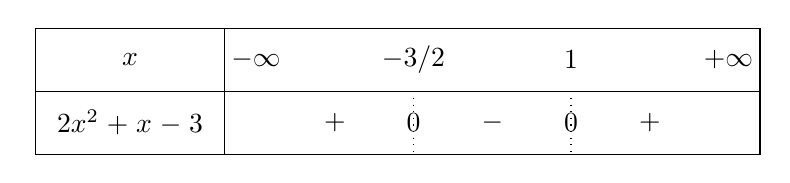
\begin{tikzpicture}[scale=0.8]
   \tkzTabInit[lgt = 3, espcl = 2.5]{$x$ / 1 ,$2x^2+x-3$/1}{$-\infty$, $-3/2$, $1$, $+\infty$}
      \tkzTabLine{, +,z,-,z,+,  }
\end{tikzpicture}
\end{center}

Ainsi, $\displaystyle\lim_{x \to \left(-\frac{3}{2}\right)^-}(2x^2+x-3)=0^+$ et $\displaystyle\lim_{x \to \left(-\frac{3}{2}\right)^-}(x^2-4x-12)=-\dfrac{15}{4}$. Ainsi, $\displaystyle\lim_{x \to \left(-\frac{3}{2}\right)^-}f(x)=-\infty$.

Puis $\displaystyle\lim_{x \to \left(-\frac{3}{2}\right)^+}(2x^2+x-3)=0^-$ et $\displaystyle\lim_{x \to \left(-\frac{3}{2}\right)^+}(x^2-4x-12)=-\dfrac{15}{4}$. Ainsi, $\displaystyle\lim_{x \to \left(-\frac{3}{2}\right)^+}f(x)=+\infty$.

Par ailleurs, $\displaystyle\lim_{x \to \left(1\right)^-}(2x^2+x-3)=0^-$ et $\displaystyle\lim_{x \to \left(1\right)^-}(x^2-4x-12)=-15$. Ainsi, $\displaystyle\lim_{x \to \left(1\right)^-}f(x)=+\infty$.

Enfin, $\displaystyle\lim_{x \to \left(1\right)^+}(2x^2+x-3)=0^+$ et $\displaystyle\lim_{x \to \left(1\right)^+}(x^2-4x-12)=-15$. Ainsi, $\displaystyle\lim_{x \to \left(1\right)^+}f(x)=-\infty$.

\item $f$ est le quotient de deux fonctions dérivables sur chaque intervalle de $D$, et dont le dénominateur ne s'annule pas sur $D$. $f$ est donc dérivable sur chaque intervalle de $D$. Pour tout réel $x\in D$, on a alors
\[f'(x)=\dfrac{(2x-4)(2x^2+x-3)-(x^2-4x-12)(4x+1)}{(2x^2+x-3)^2}=\dfrac{9x^2+42x+24}{(2x^2+x-3)^2}.\]
\item Pour tout $x\in D$, $(2x^2+x-3)^2>0$. $f'(x)$ est donc du signe de $9x^2+42x+24$. Il s'agit d'un polynôme du second degré dont les racines sont $-4$ et $-\dfrac{2}{3}$. On peut alors construire le tableau de signes de $f'$ et en déduire les variations de $f$.

\begin{center}
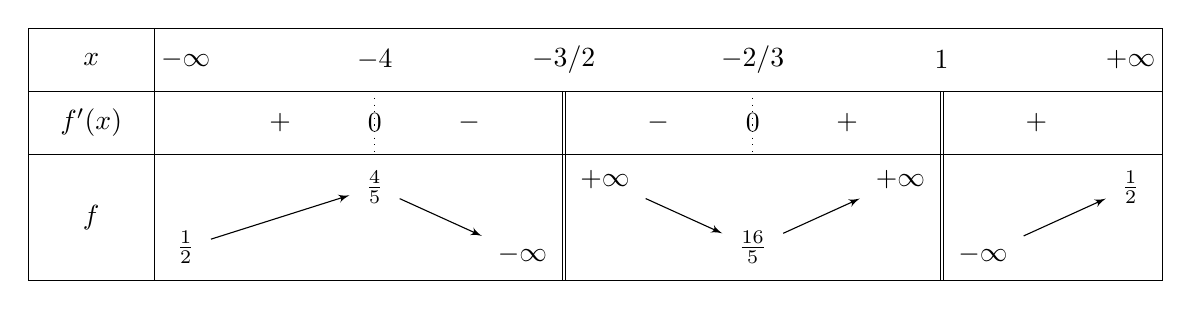
\begin{tikzpicture}[scale=0.8]
   \tkzTabInit{$x$ / 1 ,$f'(x)$/1,$f$/2}{$-\infty$, $-4$, $-3/2$, $-2/3$, $1$ ,$+\infty$}
      \tkzTabLine{,+,z,-, d,- ,z,+,d,+,  }
   \tkzTabVar{-/$\frac{1}{2}$,+/$\frac{4}{5}$,-D+/$-\infty$/$+\infty$,-/$\frac{16}{5}$,+D-/$+\infty$/$-\infty$,+/$\frac{1}{2}$}
\end{tikzpicture}
\end{center}

\begin{center}
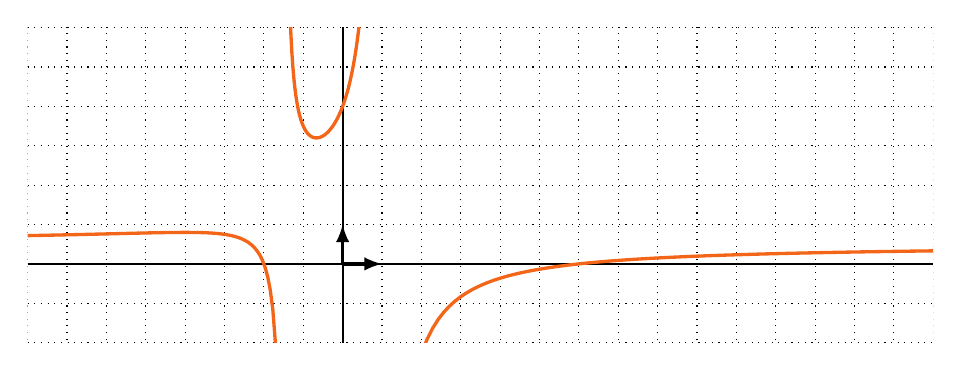
\begin{tikzpicture}[scale=0.5]
\clip (-8,-2) rectangle (15,6);
\draw [thin, dotted] (-8,-8) grid (15,8);
\draw [thick] (-8,0)--(15,0);
\draw [thick] (0,-8) -- (0,8);
\draw [very thick,->,>=latex] (0,0)--(0,1);
\draw [very thick,->,>=latex] (0,0)--(1,0);
\draw [very thick, ocre,domain=-8:-1.51,samples=100] plot (\x,{(\x*\x-4*\x-12)/(2*\x*\x+\x-3)});
\draw [very thick, ocre,domain=-1.49:0.99,samples=100] plot (\x,{(\x*\x-4*\x-12)/(2*\x*\x+\x-3)});
\draw [very thick, ocre,domain=1.01:15,samples=100] plot (\x,{(\x*\x-4*\x-12)/(2*\x*\x+\x-3)});
\end{tikzpicture}
\end{center}
\end{enumerate}

\end{solution}





\begin{exercise}[topic=lim22]On considère la fonction $f:x\mapsto \dfrac{\sqrt{x^2-3x+2}}{x+1}$
\begin{enumerate}
\item Donner le domaine de définition de $f$.
\item Déterminer les limites éventuelles de $f$ en $-\infty$, $+\infty$, $-1^+$ et $-1^-$.
\end{enumerate}
\end{exercise}

\begin{solution}$\sqrt{x^2-3x+2}$ existe si et seulement si $x^2-3x+2\geqslant 0$. Or, $x^2-3x+2$ est un polynôme du second degré dont les racines sont 1 et 2.

\begin{center}
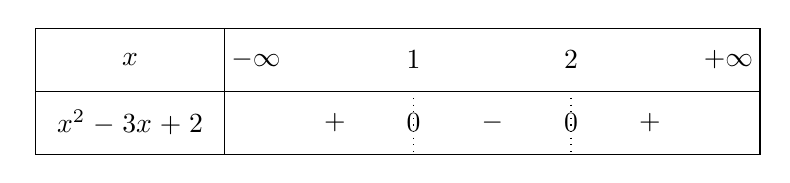
\begin{tikzpicture}[scale=0.8]
   \tkzTabInit[lgt = 3, espcl = 2.5]{$x$ / 1 ,$x^2-3x+2$/1}{$-\infty$, $1$, $2$, $+\infty$}
      \tkzTabLine{, +,z,-,z,+,  }
\end{tikzpicture}
\end{center}

Ainsi, $\sqrt{x^2-3x+2}$ existe pour $x\in ]-\infty;1]\cup[2;+\infty[$. Par ailleurs, $-1$ est une valeur interdite puisqu'elle annule le dénominateur de $f$. Ainsi, le domaine de définition de $f$ est $(]-\infty;1]\cup[2;+\infty[) \setminus\{-1\}$.

Pour tout réel $x>2$, $\sqrt{x^2}=x$ et donc $\sqrt{x^2-3x+2}=\sqrt{x^2} \times \sqrt{1-\dfrac{3}{x}+\dfrac{2}{x^2}} =x\sqrt{1-\dfrac{3}{x}+\dfrac{2}{x^2}}$. 

Ainsi, pour tout $x>2$, $f(x)=\dfrac{x\sqrt{1-\dfrac{3}{x}+\dfrac{2}{x^2}}}{x\left(1+\dfrac{1}{x}\right)} = \dfrac{\sqrt{1-\dfrac{3}{x}+\dfrac{2}{x^2}}}{\left(1+\dfrac{1}{x}\right)}$.\\
Il en vient que $\displaystyle\lim_{x \to +\infty}f(x)=1$. 

Par ailleurs, pour tout réel $x<-1$, $\sqrt{x^2}=-x$ ! Il faut bien faire attention au signe ici. 

Ainsi, pour tout réel $x<-1$, $f(x)=\dfrac{-x\sqrt{1-\dfrac{3}{x}+\dfrac{2}{x^2}}}{x\left(1+\dfrac{1}{x}\right)} = \dfrac{-\sqrt{1-\dfrac{3}{x}+\dfrac{2}{x^2}}}{\left(1+\dfrac{1}{x}\right)}$.\\
Il en vient que $\displaystyle\lim_{x \to +\infty}f(x)=-1$. 

Puis, $\displaystyle\lim_{x\to (-1)^-}(x^2-3x+2)=\sqrt{6}>0$. De plus, si $x<-1$, alors $1+x<0$. Ainsi, $\displaystyle\lim_{x\to (-1)^-}(1+x)=0^-$ et $\displaystyle\lim_{x\to (-1)^-}f(x)=-\infty$.

Enfin, $\displaystyle\lim_{x\to (-1)^+}(x^2-3x+2)=\sqrt{6}>0$. De plus, si $x>-1$, alors $1+x>0$. \\On en déduit que $\displaystyle\lim_{x\to (-1)^+}(1+x)=0^+$. Ainsi, $\displaystyle\lim_{x\to (-1)^+}f(x)=+\infty$.\end{solution}







\begin{exercise}[topic=lim22] Une autre forme indéterminée...
\begin{enumerate}
\item Trouver trois réels $a$, $b$ et $c$ tels que, pour tout réel $x$, \(2x^3+6x^2-9x+1=(x-1)(ax^2+bx+c)\)	.
\item En déduire $\displaystyle \lim_{x \to 1} \dfrac{2x^3+6x^2-9x+1}{3x^2-x-2}$.
\end{enumerate}\end{exercise}

\begin{solution}On développe l'expression de droite. Pour tout réel $x$,
\[(x-1)(ax^2+bx+c) = ax^3+(b-a)x^2+(c-b)x-c.\]
On identifie alors les coefficients de $2x^3+6x^2-9x+1$ et $ax^3+(b-a)x^2+(c-b)x-c$. Il suffit de trouver $a$, $b$ et $c$ tel que $a=2$, $b-a=6$, $c-b=-9$ et $-c=1$. On a donc $a=2$, $c=-1$ puis $b-a=6$ et $c-b=-9$.

En prenant $a=2$, $b=8$ et $c=-1$, on a alors $(x-1)(2x^2+8x-1)(x-1)=2x^3+6x^2-9x+1$.

Les racines du polynôme $3x^2-x-2$ sont 1 et $-\dfrac{2}{3}$. Ainsi, pour tout réel $x$, $3x^2-x-2=3(x-1)\left(x+\dfrac{2}{3}\right)$. 

Alors, pour tout réel $x$ différent de $1$ et $-\dfrac{2}{3}$, $\dfrac{2x^3+6x^2-9x+1}{3x^2-x-2}=\dfrac{(x-1)(2x^2+8x-1)}{3(x-1)\left(x+\dfrac{2}{3}\right)}=\dfrac{2x^2+8x-1}{3x+2}$.

Ainsi, $\displaystyle \lim_{x \to 1} \dfrac{2x^3+6x^2-9x+1}{3x^2-x-2}=\dfrac{2\times 1^2+8\times 1 -1}{3 \times 1 +2 }=\dfrac{9}{5}$.\end{solution}





\begin{exercise}[topic=lim22]

On rappelle qu'une fonction $f$ est dérivable en $x$ si le taux de variation $\dfrac{f(x+h)-f(x)}{h}$ admet une limite finie lorsque $h$ tend vers 0.

\begin{enumerate}
\item Écrire le taux de variations de la fonction $f:x\mapsto \e^x$ entre 0 et $h$.
\item Que vaut $f'(0)$ ? En déduire la valeur de $\displaystyle \lim_{x \to 0} \dfrac{\e^x-1}{x}$
\end{enumerate}\end{exercise}

\begin{solution}Ce taux vaut $\dfrac{\e^h-\e^0}{h-0}$ soit $\dfrac{\e^h-1}{h}$.

$f'(0)=\e^0=1$. Ainsi, par définition de la dérivée, $\displaystyle \lim_{x \to 0} \dfrac{\e^x-1}{x} = 1$.\end{solution}

\printcollection{lim22}

\section*{Comparaison de limites}

\begin{exercise}[topic=lim23]Déterminer les limites suivantes.

\renewcommand{\arraystretch}{1.5}
\begin{tabularx}{\linewidth}{XXX}
 \textbf{a.} $\displaystyle \lim_{x \to +\infty} (\e^x + \sin(x))$ &
 \textbf{b.} $\displaystyle \lim_{x \to +\infty} \left(x^2+\dfrac{3}{x}\right)$ &
  \textbf{c.} $\displaystyle \lim_{x \to +\infty} \sqrt{x^2+1}$ \\
 \textbf{d.} $\displaystyle \lim_{x \to -\infty} \left((\cos(4x)-3)x^3\right)$ & 
 \textbf{e.} $\displaystyle \lim_{x \to +\infty} \left((\cos(4x)-3)x^3\right)$ &
 \textbf{f.}  $\displaystyle \lim_{x \to +\infty} \dfrac{3\sin(x)+2 \cos(x)}{x^3}$ \\
 \textbf{g.} $\displaystyle \lim_{x \to +\infty} \left(1+\dfrac{\sin (x)}{\sqrt{x}}\right)$ &
  \textbf{h.} $\displaystyle \lim_{x \to +\infty} \left( \dfrac{x+2\sin(x)}{x}\right)$ & 
 \textbf{i.} $\displaystyle \lim_{x \to -\infty} \left(\dfrac{x+2\sin (x)}{x}\right)$ \\
  \textbf{j.} $\displaystyle \lim_{x \to +\infty} \dfrac{x+\cos(x)}{x+\sin(x)}$ &
 \textbf{k.} $\displaystyle \lim_{x \to +\infty}\sqrt{x+\sin(x)+3}$ & 
 \textbf{l.} $\displaystyle \lim_{x \to +\infty}2x^2-3x+\sin(4x)$
\end{tabularx}\end{exercise}

\begin{solution}\textbf{a.} Pour tout réel $x$, $\e^x+\sin(x) \geqslant \e^x -1$. Or, $\displaystyle \lim_{x \to + \infty}(\e^x-1)=+\infty$.\\ Ainsi, par comparaison, $\displaystyle \lim _{x\to + \infty}(\e^x + \sin (x))=+\infty$.

 \textbf{b.} Pour tout réel $x>0$, $x^2+\dfrac{3}{x}\geqslant x^2$ Or, $\displaystyle \lim_{x \to +\infty}x^2=+\infty$. Ainsi, par comparaison, $\displaystyle \lim_{x \to +\infty} \left(x^2+\dfrac{3}{x}\right)=+\infty$. Il est évidemment possible de faire une simple somme de limites. 

 \textbf{c.} Pour tout réel $x>0$, $x^2+1 \geqslant x^2$, d'où $\sqrt{x^2+1} \geqslant \sqrt{x^2}$, c'est-à-dire $f(x)\geqslant x$ Or, $\displaystyle \lim_{x \to +\infty}x=+\infty$. Ainsi, par comparaison, $\displaystyle \lim_{x \to +\infty} \sqrt{x^2+1}=+\infty$.
 
  \textbf{d.} Pour tout réel $x$, $-1\leqslant \cos(4x) \leqslant 1$. Ainsi, $-4 \leqslant \cos(4x)-3 \leqslant -2$. En particulier, pour $x>0$, $f(x) \leqslant -2x^3$. Or, $\displaystyle\lim _{x \to +\infty} (-2x^3)=-\infty$. Ainsi, par comparaison,  $\displaystyle \lim_{x \to +\infty} \left((\cos(4x)-3)x^3\right)=-\infty$.

 \textbf{e.} Par ailleurs, pour $x<0$, on a $\left((\cos(4x)-3)x^3\right) \geqslant -4x^3$. Or, $\displaystyle \lim_{x \to -\infty} (-4x^3)=+\infty$.\\ Ainsi, $\displaystyle \lim_{x \to -\infty} \left((\cos(4x)-3)x^3\right)=+\infty$.

 \textbf{f.} Pour tout réel $x>0$, $-3  \leqslant 3\sin(x) \leqslant 3$ et $-2\leqslant 2\cos(x)\leqslant 2$. \\ Ainsi, pour tout réel $x$, $-5\leqslant 3\sin(x)+2\cos(x) \leqslant 5$ et donc $-\dfrac{5}{x^3} \leqslant \dfrac{3\sin(x)+2\cos(x)}{x^3} \leqslant \dfrac{5}{x^3}$. \\ Or, $\displaystyle\lim_{x\to+\infty}\left(-\dfrac{5}{x^3}\right) = \displaystyle\lim_{x\to+\infty}\left(\dfrac{5}{x^3}\right)=0$. Par encadrement, $\displaystyle\lim_{x\to+\infty}\left(\dfrac{3\sin(x)+2\cos(x)}{x^3}\right)=0$.
 
\textbf{g.} Pour tout réel $x>0$, $-1 \leqslant \sin(x) \leqslant 1$ et donc $-\dfrac{1}{\sqrt{x}} \leqslant \dfrac{\sin(x)}{\sqrt{x}} \leqslant \dfrac{1}{\sqrt{x}}$. \\ Or, $\displaystyle\lim_{x\to+\infty}\left(-\dfrac{1}{\sqrt{x}}\right)=\displaystyle\lim_{x\to+\infty}\left(\dfrac{1}{\sqrt{x}}\right)=0$. Ainsi, d'après le théorème d'encadrement, $\displaystyle\lim_{x\to+\infty}\left(\dfrac{\sin(x)}{\sqrt{x}}\right)=0$ et donc $\displaystyle\lim_{x\to+\infty}\left(1+\dfrac{\sin(x)}{\sqrt{x}}\right)=1$.
  
\textbf{h.} Pour tout réel $x\neq 0$, $\dfrac{x+2\sin(x)}{x}=1+2\dfrac{\sin(x)}{x}$. Or, pour tout $x>0$, $-\dfrac{1}{x} \leqslant \dfrac{\sin(x)}{x} \leqslant \dfrac{1}{x}$.\\ Or, $\displaystyle\lim_{x\to+\infty}\left(-\dfrac{1}{x}\right)=\displaystyle\lim_{x\to+\infty}\dfrac{1}{x}=0$. D'après le théorème d'encadrement, $\displaystyle\lim_{x\to+\infty}\dfrac{\sin(x)}{x}=0$ et donc \\ $\displaystyle\lim_{x\to+\infty}\left(\dfrac{x+2\sin(x)}{x}\right)=1$.
   
\textbf{i.} Pour tout réel $x\neq 0$, $\dfrac{x+2\sin(x)}{x}=1+2\dfrac{\sin(x)}{x}$.\\ Or, pour tout $x<0$, $-1 \leqslant \sin(x)\leqslant 1$ et donc $-\dfrac{1}{x} \geqslant \dfrac{\sin(x)}{x} \geqslant \dfrac{1}{x}$ ($x$ est négatif, attention à bien changer le sens de l'inégalité !). Or, $\displaystyle\lim_{x\to-\infty}\left(-\dfrac{1}{x}\right)=\displaystyle\lim_{x\to-\infty}\dfrac{1}{x}=0$. \\ D'après le théorème d'encadrement, $\displaystyle\lim_{x\to-\infty}\dfrac{\sin(x)}{x}=0$ et donc $\displaystyle\lim_{x\to-\infty}\left(\dfrac{x+2\sin(x)}{x}\right)=1$.
    
\textbf{j.} Pour tout réel $x>0$, $\dfrac{x+\cos(x)}{x+\sin(x)}=\dfrac{x}{x}\times \dfrac{1+\dfrac{\cos(x)}{x}}{1+\dfrac{\sin(x)}{x}}=\dfrac{1+\dfrac{\cos(x)}{x}}{1+\dfrac{\sin(x)}{x}}$.

Or, pour tout réel $x>0$, $-\dfrac{1}{x} \leqslant \dfrac{\cos(x)}{x}\leqslant \dfrac{1}{x}$ et $-\dfrac{1}{x} \leqslant \dfrac{\sin(x)}{x}\leqslant \dfrac{1}{x}$. Or, $\displaystyle\lim_{x\to +\infty}\left(-\dfrac{1}{x}\right)=\displaystyle\lim_{x\to +\infty}\left(\dfrac{1}{x}\right)=0$. Ainsi, d'après le théorème d'encadrement, $\displaystyle\lim_{x\to +\infty}\left(\dfrac{\cos(x)}{x}\right)=0$ et $\displaystyle\lim_{x\to +\infty}\left(\dfrac{\sin(x)}{x}\right)=0$. \\ Ainsi, $\displaystyle\lim_{x\to +\infty}\left(\dfrac{x+\cos(x)}{x+\sin(x)}\right)=1$.
     
\textbf{k.}Pour tout réel $x>0$, $x+\sin(x)+3 \geqslant x+2$. Par croissance de la fonction racine carrée sur $[0;+\infty[$, il en vient que $\sqrt{x+\sin(x)+3}\geqslant \sqrt{x+2}$. Or, $\displaystyle\lim_{x\to+\infty}\sqrt{x+2}=+\infty$.\\  Par comparaison, $\displaystyle\lim_{x\to+\infty}\sqrt{x+\sin(x)+3}=+\infty$.
      
\textbf{l.} Pour tout réel $x>0$, $2x^2-3x+\sin(4x)\geqslant 2x^2-3x-1$. \\ Or, pour tout réel $x>0$, $2x^2-3x-1 =x^2\left(2-\dfrac{3}{x}-\dfrac{1}{x^2}\right)$. Ainsi, $\displaystyle\lim_{x\to +\infty}(2x^2-3x-1)=+\infty$.\\ Par comparaison, $\displaystyle\lim_{x\to +\infty}(2x^2-3x+\sin(4x))=+\infty$.
 
 \end{solution}
 
 



\begin{exercise}[topic=lim23] Déterminer les limites suivantes.
\renewcommand{\arraystretch}{2.5}

\begin{tabularx}{\linewidth}{XXX}
 \textbf{a.} $\displaystyle \lim_{x \to +\infty} x^5\e^{-x}$ & \textbf{b.} $\displaystyle \lim_{x \to -\infty} x^5\e^{-x}$ &
 \textbf{c.} $\displaystyle \lim_{x \to +\infty} \dfrac{\e^{4x}}{x^2}$ \\

 \textbf{d.} $\displaystyle \lim_{x \to +\infty} \dfrac{\e^x-1}{\e^x+x}$ &  \textbf{e.} $\displaystyle \lim_{x \to -\infty} \dfrac{\e^x-1}{\e^x+x}$ &
  \textbf{f.} $\displaystyle \lim_{x \to +\infty} \dfrac{3x\e^x+4\e^x+3x}{\e^{2x}+\e^x+1}$ \\
 
 \textbf{g.}  $\displaystyle \lim_{x \to -\infty} \dfrac{3x\e^x+4\e^x+3x}{\e^{2x}+\e^x+1}$ &
 \textbf{h.} $\displaystyle \lim_{x \to +\infty} \dfrac{\e^{3x}}{28x}$ & \textbf{i.} $\displaystyle \lim_{x \to -\infty} \dfrac{\e^{3x}}{28x}$ \\
 
  \textbf{j.} $\displaystyle \lim_{x \to +\infty}(\e^x - 3x^2+5x-1)$ &  \textbf{k.} $\displaystyle \lim_{x \to -\infty}(\e^x - 3x^2+5x-1)$ &
 \textbf{l.} $\displaystyle \lim_{x \to +\infty} \dfrac{\e^x+\e^{-x}}{x}$ \\
  \textbf{m.}  $\displaystyle \lim_{x \to -\infty} \dfrac{\e^x+\e^{-x}}{x}$ &
 \textbf{n.}  $\displaystyle \lim_{x \to 0^+} \dfrac{\e^x+\e^{-x}}{x}$ &  \textbf{o.}  $\displaystyle \lim_{x \to 0^-} \dfrac{\e^x+\e^{-x}}{x}$ \\
  
 \textbf{p.}   $\displaystyle \lim_{x \to +\infty} \dfrac{(2+\cos(x))\e^x}{x}$ &  \textbf{q.}  $\displaystyle \lim_{x \to -\infty} \dfrac{(2+\cos(x))\e^x}{x}$ &
   
 \textbf{r.}    $\displaystyle \lim_{x \to +\infty}( x^2\e^{-x}-x)$ 
 
\end{tabularx}\end{exercise}

\begin{solution}  

\textbf{a.} Par croissances comparées, $\displaystyle\lim_{x\to+\infty}x^5\e^{-x}=0$.

\textbf{b.} On a $\displaystyle\lim_{x\to-\infty}x^5 = -\infty$ et $\displaystyle\lim_{x\to -\infty}\e^{-x}=+\infty$.  Par produit, $\displaystyle\lim_{x\to -\infty}x^5\e^{-x}=-\infty$.

\textbf{c.} Pour tout réel $x>0$, $\dfrac{\e^{4x}}{x^2} = 16 \times \dfrac{\e^{4x}}{(4x)^2}$. \\ Or, $\displaystyle\lim_{x\to +\infty}4x=+\infty$ et, par croissances comparées, $\displaystyle\lim_{X \to +\infty} \dfrac{\e^X}{X^2}=+\infty$. Ainsi, $\displaystyle\lim_{x\to+\infty}\dfrac{\e^{4x}}{x^2}=+\infty$.

\textbf{d.} Pour tout réel $x$, $\dfrac{\e^x-1}{\e^x+x}=\dfrac{\e^x\left(1-\dfrac{1}{\e^x}\right)}{\e^x\left(1+\dfrac{x}{\e^x}\right)}=\dfrac{1-\dfrac{1}{\e^x}}{1+\dfrac{x}{\e^x}}$. \\Or, $\displaystyle \lim_{x \to + \infty} \dfrac{1}{\e^x}=0$ et, par croissances comparées, $\displaystyle\lim_{x\to +\infty} \dfrac{x}{\e^x}=0$. Ainsi $\displaystyle \lim_{x \to +\infty} \dfrac{\e^x-1}{\e^x+x}=1$. 

\textbf{e.} On a $\displaystyle\lim_{x\to -\infty} (\e^x-1)=-1$ et $\displaystyle\lim_{x\to-\infty}(\e^x+x)=-\infty$. Ainsi, $\displaystyle \lim_{x \to -\infty} \dfrac{\e^x-1}{\e^x+x}=0$.


\textbf{f.} Pour tout réel non nul $x$, 
\[ \dfrac{3x\e^x+4\e^x+3x}{\e^{2x}+\e^x+1}=\dfrac{x\e^x \left(3+\dfrac{4}{x}+\dfrac{3}{\e^x}\right)}{\e^2x\left(1+\dfrac{1}{\e^x}+\dfrac{1}{\e^{2x}}\right)}=\dfrac{x}{\e^x}\times \dfrac{3+\dfrac{4}{x}+\dfrac{3}{\e^x}}{1+\dfrac{1}{\e^x}+\dfrac{1}{\e^{2x}}}.\]
$\displaystyle \lim_{x \to +\infty} \dfrac{3+\dfrac{4}{x}+\dfrac{3}{\e^x}}{1+\dfrac{1}{\e^x}+\dfrac{1}{\e^{2x}}} = 3$ et, par croissances comparées, $\displaystyle\lim_{x\to +\infty} \dfrac{x}{\e^x}=0$. Ainsi,
$\displaystyle \lim_{x \to +\infty} \dfrac{3x\e^x+4\e^x+3x}{\e^{2x}+\e^x+1}=0$.

\textbf{g.} Par ailleurs, $\displaystyle\lim_{x \to - \infty}(\e^{2x}+\e^x+1)=1$ et $\displaystyle\lim_{x \to - \infty}(3x\e^x+4\e^x+3x)=-\infty$.\\ Ainsi, $\displaystyle \lim_{x \to -\infty} \dfrac{3x\e^x+4\e^x+3x}{\e^{2x}+\e^x+1}=-\infty$.
  
\textbf{h.} Pour tout réel $x>0$, $\dfrac{\e^{3x}}{28x}=\dfrac{3}{28} \times \dfrac{\e^{3x}}{3x}$. Or, par croissances comparées, $\displaystyle\lim _{x\to + \infty} \dfrac{\e^{3x}}{3x}=+\infty$ .\\ Ainsi, $\displaystyle\lim _{x\to + \infty} \dfrac{\e^{3x}}{28x}=+\infty$. 

\textbf{i.} On a $\displaystyle\lim _{x\to - \infty}\e^{3x}=0$ et $\displaystyle\lim _{x\to - \infty} 28x=-\infty$. Ainsi, $\displaystyle\lim _{x\to - \infty} \dfrac{\e^{3x}}{28x}=0$. 

\textbf{j.} Pour tout réel $x$, $\e^x - 3x^2+5x-1=\e^x\left(1-3\dfrac{x^2}{\e^x}+5\dfrac{x}{\e^x}-\dfrac{1}{\e^x}\right)$ Or, $\displaystyle\lim _{x\to + \infty} \left( 1-\dfrac{3x^2}{\e^x}+5\dfrac{x}{\e^x}-\dfrac{1}{\e^x}\right)=1$ par croissances comparées. Ainsi, $\displaystyle\lim _{x\to + \infty}(\e^x - 3x^2+5x-1)=+\infty$. 

\textbf{k.} Par ailleurs, en faisant simplement la règle de somme de limites, on obtient, $\displaystyle\lim _{x\to - \infty}(\e^x - 3x^2+5x-1)=-\infty$.
 
\textbf{l.} Pour tout réel $x>0$, $\e^{-x}>0$. Ainsi, $\e^x+\e^{-x}>\e^x$ et $\dfrac{\e^x+\e^{-x}}{x}>\dfrac{\e^x}{x}$. Or, par croissances comparées, $\displaystyle \lim_{x \to +\infty} \dfrac{\e^x}{x}=+\infty$ et donc, par comparaison, $\displaystyle \lim_{x \to +\infty} \dfrac{\e^x+\e^{-x}}{x}=+\infty$.

\textbf{m.} Pour tout réel $x<0$, $\e^x>0$. Ainsi, $\e^x+\e^{-x}>\e^{-x}$. En divisant par $-x$ qui est positif, on a alors $-\dfrac{\e^x+\e^{-x}}{x}> \dfrac{\e^{-x}}{-x}$. Or,$\displaystyle \lim_{x \to -\infty }(-x)=+\infty$ et par croissances comparées, $\displaystyle \lim_{X \to +\infty} \dfrac{\e^X}{X}=+\infty$. Ainsi, $\displaystyle \lim_{x \to -\infty} \dfrac{\e^{-x}}{-x}=+\infty$. Par comparaison, on a donc, $\displaystyle \lim_{x \to -\infty} \left(-\dfrac{\e^x+\e^{-x}}{x}\right)=+\infty$ et $\displaystyle \lim_{x \to -\infty} \left(\dfrac{\e^x+\e^{-x}}{x}\right)=-\infty$.

\textbf{n.} Puisque $\displaystyle \lim_{x \to 0} (\e^x+\e^{-x})=\e^0+\e^0=2$, on a $\displaystyle \lim_{x \to 0^+} \dfrac{\e^x+\e^{-x}}{x} = +\infty$.

\textbf{o.} Puisque $\displaystyle \lim_{x \to 0} (\e^x+\e^{-x})=\e^0+\e^0=2$, on a $\displaystyle \lim_{x \to 0^-} \dfrac{\e^x+\e^{-x}}{x} = -\infty$.

\textbf{p.} Pour tout réel $x$, $\e^x \leqslant (2+\cos(x))\e^x \leqslant 3\e^x$.
 
 Pour tout réel $x>0$, on a donc $\dfrac{\e^x}{x} \leqslant \dfrac{(2+\cos(x))\e^x}{x}$. Or, par croissances comparées, $\displaystyle \lim_{x \to +\infty} \dfrac{\e^x}{x}=+\infty$. \\ Par comparaison, on a donc $\displaystyle \lim_{x \to +\infty}\dfrac{(2+\cos(x))\e^x}{x}=+\infty$.
 
\textbf{q.} Par ailleurs, pour tout réel $x<0$, on a $\dfrac{\e^x}{x} \geqslant \dfrac{(2+\cos(x))\e^x}{x}\geqslant \dfrac{3\e^x}{x}$. Or, $\displaystyle \lim_{x \to -\infty}\dfrac{3\e^x}{x}=\displaystyle \lim_{x \to -\infty}\dfrac{\e^x}{x}=0$. \\Par encadrement, $\displaystyle \lim_{x \to -\infty}\dfrac{(2+\cos(x))\e^x}{x}$ existe et vaut 0.

\textbf{r.}   Remarquons que pour tout réel $x$, $x^2\e^{-x}-x=\dfrac{x^2}{\e^x}-x$. Or, par croissances comparées, $\displaystyle \lim_{x\to+\infty} \dfrac{x^2}{\e^x}=0$ et donc $\displaystyle \lim_{x\to+\infty}\left(\dfrac{x^2}{\e^x}-x\right)=-\infty$.
\end{solution}






\begin{exercise}[topic=lim23]La fonction tangente hyperbolique est la fonction notée $th$ et définie pour tout réel $x$ par \[th(x)=\dfrac{\e^x-\e^{-x}}{\e^x+\e^{-x}}.\]
\begin{enumerate}
\item Déterminer $\displaystyle \lim_{x \to -\infty}th(x)$ et $\displaystyle \lim_{x \to +\infty} th(x)$.
\item Justifier que $th$ est dérivable sur $\mathbb{R}$ et que pour tout réel $x$,
\[th'(x)=\dfrac{4}{(\e^x+\e^{-x})^2}.\]
\item En déduire le tableau de variations de $th$.
\item Déterminer l'équation de la tangente à la courbe de la fonction $th$ à l'abscisse 0.
\item Dans un repère orthonormé, tracer l'allure de la courbe $th$ ainsi que sa tangente à l'abscisse .
0.\end{enumerate}\end{exercise}

\begin{solution}\hspace{0pt}
\begin{enumerate}
\item Pour tout réel $x>0$,  $th(x)=\dfrac{\e^x}{\e^x} \times \dfrac{1-\e^{-2x}}{1+\e^{-2x}} = \dfrac{1-\e^{-2x}}{1+\e^{-2x}}$.\\ Or, $\displaystyle\lim_{x\to+\infty}\e^{-2x}=0$. Ainsi, $\displaystyle\lim_{x \to +\infty}th(x)=1$.

Par ailleurs, pour tout réel $x<0$, $th(x)=\dfrac{\e^{-x}}{\e^{-x}} \times \dfrac{\e^{2x}-1}{\e^{2x}+1} = \dfrac{\e^{2x}-1}{\e^{2x}+1} $. \\Or, $\displaystyle\lim_{x\to -\infty}\e^{2x}=0$ Ainsi, $\displaystyle\lim_{x\to+\infty}th(x)=-1$.

\item $th$ est un quotient de fonctions dérivables sur $\mathbb{R}$ dont le dénominateur ne s'annule pas. Cette fonction est donc dérivable sur $\mathbb{R}$ et pour tout réel $x$,
\[th'(x)=\dfrac{(\e^x+\e^{-x})(\e^x+\e^{-x})-(\e^x-\e^{-x})(\e^x-\e^{-x})}{(\e^x+\e^{-x})^2}=\dfrac{\e^{2x}+2+\e^{-2x}-(\e^{2x}-2-\e^{-2x}}{(\e^x+\e^{-x})^2}=\dfrac{4}{(\e^x+\e^{-x})^2}.\]
\item $th$ est donc strictement croissante sur $\mathbb{R}$.
\item L'équation de la tangente à la courbe de la fonction $th$ en 0 est $y=th'(0)(x-0)+th(0)$.\\ Or, $th'(0)=\dfrac{4}{(\e^0+\e^0)^2}=1$ et $th(0)=\dfrac{\e^0-\e^0}{\e^0+\e^0}=0$. Ainsi, l'équation de cette tangente est $y=x$.
\item \begin{center}
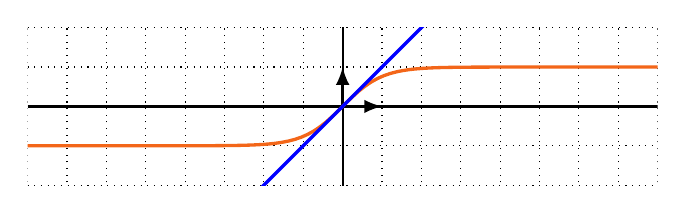
\begin{tikzpicture}[scale=0.5]
\clip (-8,-2) rectangle (8,2);
\draw [thin, dotted] (-8,-8) grid (15,8);
\draw [thick] (-8,0)--(15,0);
\draw [thick] (0,-8) -- (0,8);
\draw [very thick,->,>=latex] (0,0)--(0,1);
\draw [very thick,->,>=latex] (0,0)--(1,0);
\draw [very thick, ocre,domain=-8:8,samples=100] plot (\x,{ tanh(\x )});
\draw [very thick, blue,domain=-8:8,samples=100] plot (\x,{ \x });
\end{tikzpicture}
\end{center}
\end{enumerate}

\end{solution}




\begin{exercise}[topic=lim23]
On considère la fonction $f:x\mapsto \dfrac{\e^x}{x^2+1}$. Étudier la fonction $f$ (domaine de définition, variation, signe et limites). Esquisser sa courbe représentative dans un repère orthonormé.\end{exercise}

\begin{solution}
On considère la fonction $f:x\mapsto \dfrac{\e^x}{x^2+1}$. La fonction $f$ est définie sur $\mathbb{R}$, son dénominateur n'étant jamais nul. De plus, on a, pour tout réel $x$, $f(x)>0$. $f$ est de plus dérivable et pour tout réel $x$, 
\[ f'(x)= \dfrac{\e^x \times (x^2+1) - \e^x \times 2x}{(x^2+1)^2}=\dfrac{(x-1)^2\,\e^x}{(x^2+1)^2}\geqslant 0.\]

La fonction $f$ est donc strictement croissante sur $\mathbb{R}$ puisque sa dérivée est positive et ne s'annule qu'en un nombre fini de valeurs. La courbe de $f$ a une tangente horizontale en $1$ puisque $f'(1)=0$. Par ailleurs, pour tout réel $x\neq 0$, $f(x)=\dfrac{\e^x}{x^2} \times \dfrac{1}{1+\dfrac{1}{x^2}}$. Or, par croissance comparées, $\displaystyle\lim_{x \to +\infty} \dfrac{\e^x}{x^2}=+\infty$ et $\displaystyle\lim_{x \to -\infty} \dfrac{\e^x}{x^2}=0$. $f$ a donc les mêmes limites.

La courbe de la fonction $f$ est la suivante. La tangente horizontale en $1$ est également tracée.


\begin{center}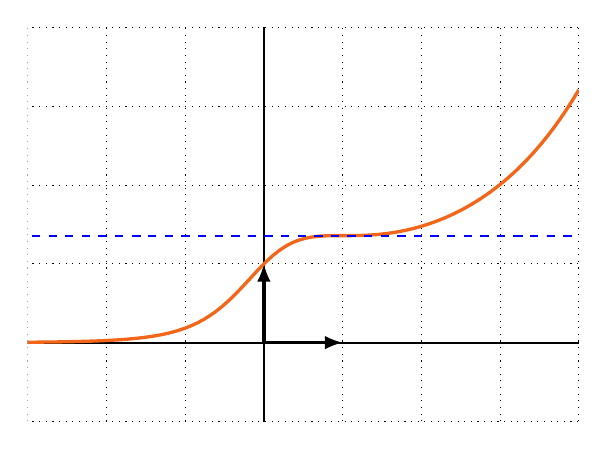
\begin{tikzpicture}[scale=1]
\clip (-3,-1) rectangle (4,4);
\draw [thin, dotted] (-8,-8) grid (15,8);
\draw [thick] (-8,0)--(15,0);
\draw [thick] (0,-8) -- (0,8);
\draw [very thick,->,>=latex] (0,0)--(0,1);
\draw [very thick,->,>=latex] (0,0)--(1,0);
\draw [very thick, ocre,domain=-4:4,samples=100] plot (\x,{(exp(\x)/(1+\x*\x)});
\draw [thick, dashed, blue,domain=-4:4,samples=100] plot (\x,{(exp(1)/(2)});

\end{tikzpicture}\end{center}

\end{solution}

\printcollection{lim23}


\section*{Approfondissement et synthèse}


\begin{exercise}[topic=lim24]
On considère la fonction $f$ définie pour tout réel $x\neq -1$ par 
\[f(x)=\dfrac{x^2+3x-4}{2x+2}.\]
\begin{enumerate}
\item Étudier la fonction $f$ : variations, signe, limites.
\item Pour tout réel $x\neq -1$, on pose $g(x)=f(x)-\left(\dfrac{1}{2}x+1\right)$.
\begin{enumerate}
\item Montrer que, pour tout réel $x\neq 2$, $g(x)=-\dfrac{6}{2x+2}$.
\item En déduire $\displaystyle \lim_{x \to +\infty} g(x)$ et $\displaystyle \lim_{x \to -\infty} g(x)$. On dit que la droite d'équation $y=\dfrac{1}{2}x+1$ est une asymptote oblique à la courbe de $f$.
\end{enumerate}
\item Dans un même repère orthonormé, tracer la droite d'équation $y=\dfrac{1}{2}x+1$ et la courbe représentative de la fonction $f$.
\end{enumerate}
\end{exercise}
\begin{solution}$f$ est définie pour tout réel $x\neq-1$.


\paragraph{Etude du signe de $f$}

$2x+2$ s'annule en $x=-1$. $x^2+3x-4$ est un polynôme du second degré dont les racines sont 1 et $-4$. On construit alors le tableau de signe de $f$.

\begin{center}
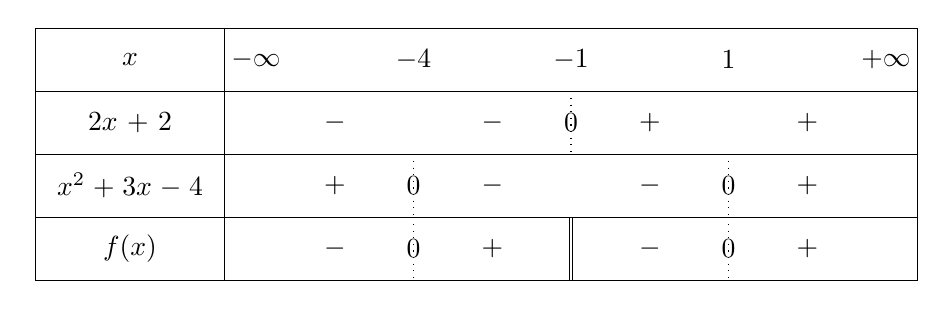
\begin{tikzpicture}[scale=0.8]
   \tkzTabInit[lgt = 3, espcl = 2.5]{$x$ / 1 ,$2x+2$/1,$x^2+3x-4$/1,$f(x)$/1}{$-\infty$, $-4$, $-1$, $1$, $+\infty$}
   \tkzTabLine{, -, ,-,z,+,, +,  }
      \tkzTabLine{, +, z,-,,-,z, +,  }
      \tkzTabLine{, -,z,+,d,-,z, +,  }
\end{tikzpicture}
\end{center}


\paragraph{Étude des limites}


Pour tout réel $x$ différent de 0 et $-1$
\[f(x)=\dfrac{x^2}{x} \times \dfrac{1+\frac{3}{x}-\dfrac{4}{x^2}}{2+\frac{2}{x}}=x \times  \dfrac{1+\frac{3}{x}-\dfrac{4}{x^2}}{2+\frac{2}{x}}.\]

Or, $\displaystyle \lim_{x \to +\infty} \dfrac{1+\frac{3}{x}-\dfrac{4}{x^2}}{2+\frac{2}{x}}=\dfrac{1}{2}$ et $\displaystyle \lim_{x \to +\infty}x=+\infty$. Ainsi, $\displaystyle \lim_{x\to +\infty}f(x)=+\infty$. De même, $\displaystyle \lim_{x\to -\infty}f(x)=-\infty$.

De plus, $\displaystyle \lim_{x \to (-1)^+} (2x+2)=0^+$ et $\displaystyle \lim_{x \to (-1)^+} (x^2+3x-4)=(-1)^2+3\times(-1)-4=-6$. En appliquant la règle des signes, on a alors $\displaystyle \lim_{x \to (-1)^+}f(x)=-\infty$.  De la même manière, $\displaystyle \lim_{x \to (-1)^-}f(x)=+\infty$.

\paragraph{Étude des variations}

Pour tout réel $x$, on pose $u(x)=x^2+3x-4$ et $v(x)=2x+2$. $u$ et $v$ sont dérivables sur $]-\infty;-1[$ et $]-1;+\infty[$ et $v$ ne s'annule pas sur ces intervalles. $f$ est donc dérivable sur ces intervalles et pour tout réel $x\neq -1$, on a
\[f'(x)=\dfrac{(2x+3)(2x+2)-(x^2+3x-4) \times 2}{(2x+2)^2}=\dfrac{x^2+2x+7}{(2x+2)^2}.\]
Puisque pour tout réel $x\neq -1$, $(2x+2)^2>0$, $f'(x)$ est du signe de $x^2+2x+7$. C'est un polynôme du second degré dont le discriminant vaut $\Delta = 2^2-4 \times 7 \times 1 = -24 >0$. Ainsi, pour tout réel $x\neq 2$, $f'(x)>0$.

\paragraph{Résumé dans un tableau}

On met toutes ces informations dans un tableau et on en profite pour vérifier si le tout est cohérent.

\begin{center}
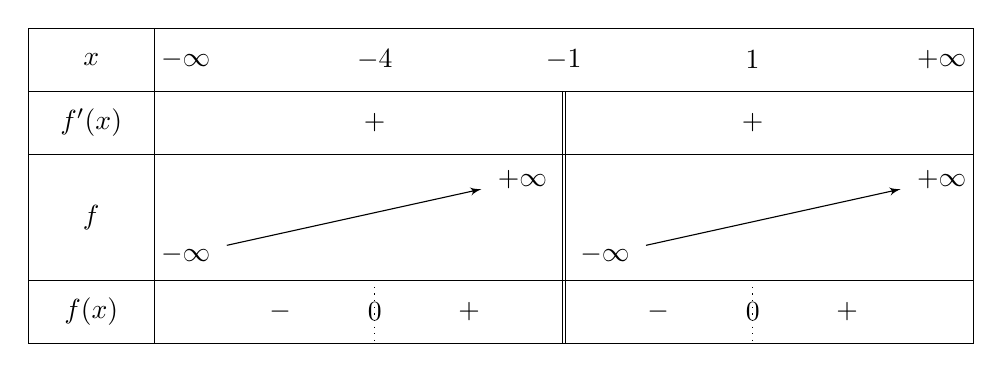
\begin{tikzpicture}[scale=0.8]
   \tkzTabInit{$x$ / 1 ,$f'(x)$/1,$f$/2,$f(x)$/1}{$-\infty$, $-4$, $-1$, $1$ ,$+\infty$}
      \tkzTabLine{, ,+,, d, ,+,  }
   \tkzTabVar{-/$-\infty$,R/,+D-/$+\infty$/$-\infty$,R/,+/$+\infty$}
   \tkzTabLine{, -,z,+,d,-,z, +,  }
\end{tikzpicture}
\end{center}

Pour tout réel $x\neq -1$, 
\[ \dfrac{x^2+3x-4}{2x+2} - \left(\dfrac{1}{2}x+1\right)=\dfrac{x^2+3x-4-\left(\dfrac{1}{2}x+1\right)(2x+2)}{2x+2}.\]
Ainsi,
\[g(x)=\dfrac{x^2+3x-4-x^2-x-2x-2}{2x+2}=-\dfrac{6}{2x+2}\]
Ainsi, $\displaystyle\lim_{x \to +\infty} \left(\dfrac{x^2+3x-4}{2x+2} - \left(\dfrac{1}{2}x+1\right)\right)=0$ et $\displaystyle\lim_{x \to -\infty} \left(\dfrac{x^2+3x-4}{2x+2} - \left(\dfrac{1}{2}x+1\right)\right)=0$.

\begin{center}
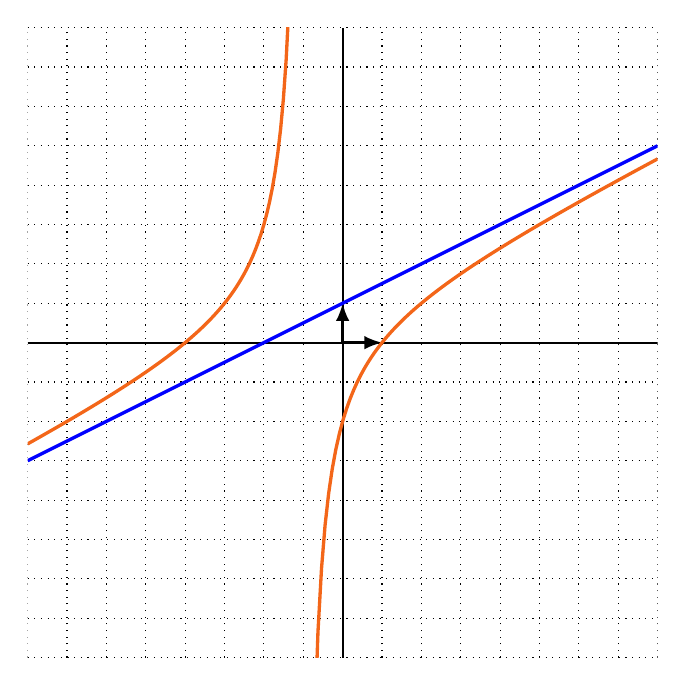
\begin{tikzpicture}[scale=0.5]
\clip (-8,-8) rectangle (8,8);
\draw [thin, dotted] (-8,-8) grid (8,8);
\draw [thick] (-8,0)--(8,0);
\draw [thick] (0,-8) -- (0,8);
\draw [very thick,->,>=latex] (0,0)--(0,1);
\draw [very thick,->,>=latex] (0,0)--(1,0);
\draw [very thick, ocre,domain=-8:-1.01,samples=100] plot (\x,{(\x*\x+3*\x-4)/(2*\x+2)});
\draw [very thick, ocre,domain=-0.99:8,samples=100] plot (\x,{(\x*\x+3*\x-4)/(2*\x+2)});
\draw [very thick, blue,domain=-8:8,samples=100] plot (\x,{\x/2+1});
\end{tikzpicture}
\end{center}

\end{solution}




\begin{exercise}[topic=lim24]On considère la fonction $f$ définie pour tout réel $x \neq 1$ par $f(x)=\dfrac{x^2}{x-1}$.
\begin{enumerate}
\item Déterminer trois réels $a$, $b$ et $c$ tels que, pour tout réel $x\neq 1$, 
\[f(x)=ax+b+\dfrac{c}{x-1}.\]
\item En déduire que la courbe de $f$ admet une asymptote oblique en $+\infty$ et en $-\infty$ dont on déterminera l'équation.
\end{enumerate}\end{exercise}

\begin{solution}Pour tout réel $x$, 
\[ax+b+\dfrac{c}{x-1}=\dfrac{ax(x-1)+b(x-1)+c}{x-1}=\dfrac{ax^2+(b-a)x+c-b}{x-1}.\]
On cherche donc $a$, $b$ et $c$ tels que $a=1$, $b-a=0$ et $c-b=0$ : on trouve $a=b=1$.\\ Ainsi, pour tout réel $x$, $\dfrac{x^2}{x-1}=x+1+\dfrac{1}{x-1}$.

On a alors $\displaystyle\lim_{x\to +\infty}(f(x)-(x+1))=\displaystyle\lim_{x\to +\infty}\dfrac{1}{x-1}=0$, et de même en $-\infty$. La droite d'équation $y=x+1$ est asymptote à la courbe de $f$ en $-\infty$ et $+\infty$.\end{solution}




\begin{exercise}[topic=lim24]On considère la fonction $f : x\mapsto \sqrt{x^2-3x+2}$.
\begin{enumerate}
\item Donner le domaine de définition $D$ de $f$.
\item Déterminer $\displaystyle \lim_{x \to +\infty} f(x)$ et $\displaystyle \lim_{x \to -\infty} f(x)$.
\item Étudier les variations de $f$ sur $D$.
\item Écrire le polynôme $x^2-3x+2$ sous forme canonique.
\item En déduire que la droite d'équation $y=x-\dfrac{3}{2}$ est asymptote à la courbe de $f$ en $+\infty$ et que la droite d'équation $y=\dfrac{3}{2}-x$ est asymptote à la courbe de $f$ en $-\infty$.
\item Tracer l'allure de la courbe de $f$ dans un repère orthonormé.
\end{enumerate}\newpage \end{exercise}

\begin{solution}\hspace{0pt}

\begin{enumerate}
\item $f(x)$ existe si et seulement si $x^2-3x+2\geqslant 0$. Or, $x^2-3x+2$ est un polynôme du second degré dont les racines sont $1$ et $2$. Ainsi, $f$ est définie sur $]-\infty ;1]\cup [2;+\infty[$.
\item Par somme, $\displaystyle\lim_{x \to - \infty}x^2-3x+2=+\infty$. Par ailleurs, pour tout $x>2$, $x^2-3x+2=x^2\left(1-\dfrac{3}{x}+ \dfrac{2}{x^2}\right)$ et donc $\displaystyle\lim_{x \to + \infty}x^2-3x+2=+\infty$. Or, $\displaystyle\lim_{X \to + \infty}\sqrt{X}=+\infty$.

Ainsi, $\displaystyle\lim_{x \to + \infty}f(x)=\displaystyle\lim_{x \to - \infty}f(x)=+\infty$
\item $f$ est dérivable sur $]-\infty;1[$ et $]2;+\infty[$. Pour tout réel $x$ dans l'un de ces intervalles, $f'(x)=\dfrac{2x-3}{2\sqrt{x^2-3x+2}}$ qui est du signe de $2x-3$.
\begin{center}
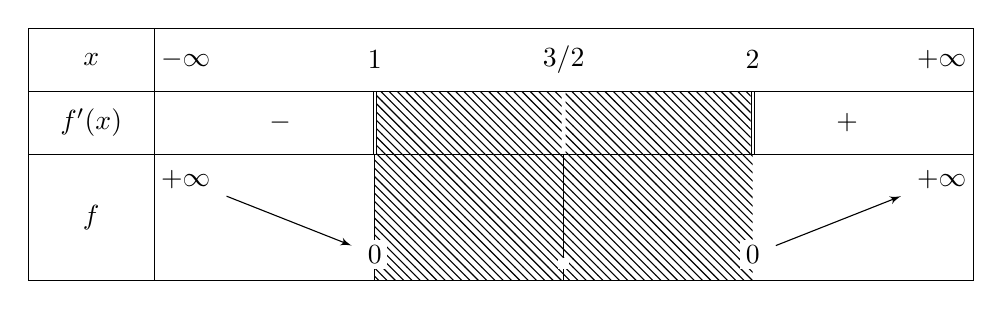
\begin{tikzpicture}[scale=0.8]
   \tkzTabInit{$x$ / 1 ,$f'(x)$/1,$f$/2}{$-\infty$, $1$, $3/2$, $2$,$+\infty$}
      \tkzTabLine{,-,d,h ,,h,d,+, }
   \tkzTabVar{+/$+\infty$,-H/$0$,-H/$ $,-/$0$,+/$+\infty$}
\end{tikzpicture}
\end{center}


\item Pour tout réel $x$, $x^2-3x+2 = \left(x-\dfrac{3}{2}\right)^2-\left(\dfrac{3}{2}\right)^2+2=\left(x-\dfrac{3}{2}\right)^2-\dfrac{1}{4}$.

\item Pour tout réel $x>2$,
\[f(x)=\sqrt{ \left(x-\dfrac{3}{2}\right)^2-\dfrac{1}{4}}= \sqrt{\left(x-\dfrac{3}{2}\right)^2} \times \sqrt{ 1-\dfrac{1}{4\left(x-\dfrac{3}{2}\right)^2}}.\]
Or, si $x>2$, alors $x-\dfrac{3}{2}>0$ et donc $\sqrt{\left(x-\dfrac{3}{2}\right)^2}=x-\dfrac{3}{2}$. Ainsi, pour tout $x>2$,
\[f(x)-\left(x-\dfrac{3}{2}\right) = \sqrt{ 1-\dfrac{1}{4\left(x-\dfrac{3}{2}\right)^2}}-1.\]
On a donc $\displaystyle\lim_{x\to+\infty}\left(f(x)-\left(x-\dfrac{3}{2}\right)\right)=0$. La droite d'équation $y=x-\dfrac{3}{2}$ est asymptote à la courbe de $f$ en $+\infty$.

Par ailleurs, pour tout $x<1$, $x-\dfrac{3}{2}<0$ et donc $\sqrt{\left(x-\dfrac{3}{2}\right)^2}=\dfrac{3}{2}-x$. Ainsi, pour tout $x<1$,
\[f(x)-\left(\dfrac{3}{2}-x\right) = \sqrt{ 1-\dfrac{1}{4\left(x-\dfrac{3}{2}\right)^2}}-1.\]
On a donc $\displaystyle\lim_{x\to-\infty}\left(f(x)-\left(\dfrac{3}{2}-x\right)\right)=0$. La droite d'équation $y=\dfrac{3}{2}-x$ est asymptote à la courbe de $f$ en $-\infty$.

\item \begin{center}
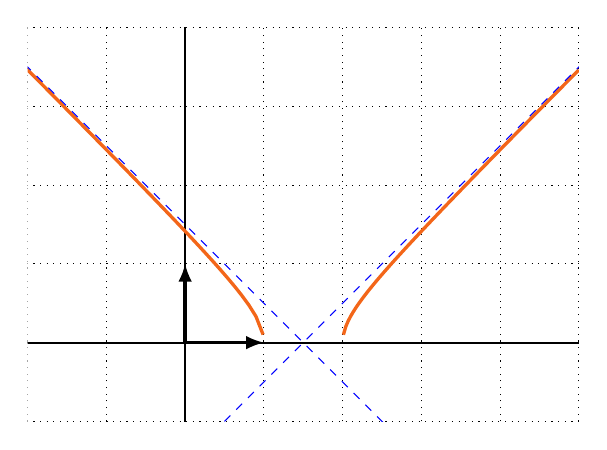
\begin{tikzpicture}[scale=1]
\clip (-2,-1) rectangle (5,4);
\draw [thin, dotted] (-8,-8) grid (8,8);
\draw [thick] (-8,0)--(8,0);
\draw [thick] (0,-8) -- (0,8);
\draw [very thick,->,>=latex] (0,0)--(0,1);
\draw [very thick,->,>=latex] (0,0)--(1,0);
\draw [very thick, ocre,domain=-8:0.99,samples=100] plot (\x,{sqrt(\x*\x-3*\x+2)});
\draw [very thick, ocre,domain=2.01:5,samples=100] plot (\x,{sqrt(\x*\x-3*\x+2)});
\draw [thin, dashed, blue,domain=-8:8,samples=100] plot (\x,{\x -3/2});
\draw [thin, dashed, blue,domain=-8:8,samples=100] plot (\x,{ 3/2-\x});
\end{tikzpicture}
\end{center}

\end{enumerate}


\end{solution}




\begin{exercise}[topic=lim24, subtitle={(Antilles - Guyane 2019)}]
Soit $a$ et $b$ deux réels. On considère une fonction $f$ définie pour tout réel $x$ sur $[0;+\infty[$ par
\[f(x)=\dfrac{a}{1+\e^{-bx}}.\]
La courbe $C_f$ représentant la fonction $f$ dans un repère orthogonal est donnée ci-dessous. Cette courbe passe par le point $A(0\, ;\, 0,5)$.
La tangente à la courbe $C_f$ au point $A$ passe par le point $B(10\,;\,1)$.
\vskip10pt
\begin{center}
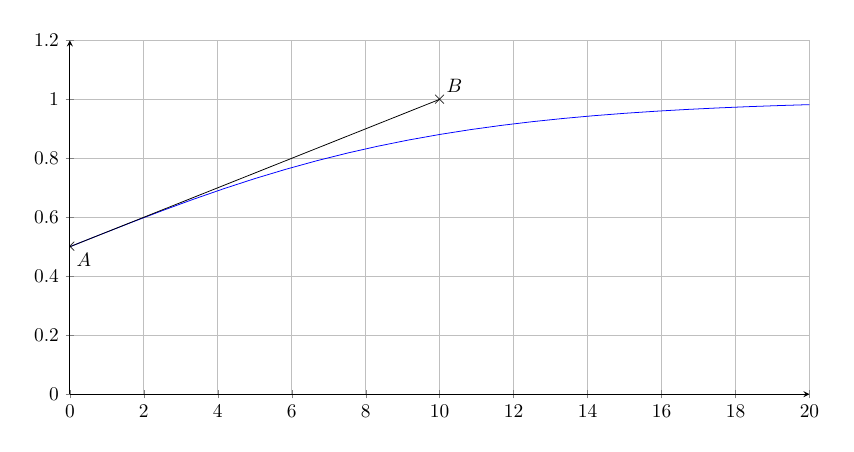
\begin{tikzpicture}[scale=0.7]
\begin{axis}[height=8cm,width=15cm,axis x line=bottom,axis y line = left, grid=major, ymin = 0, ymax = 1.2,]
\addplot expression[domain=0:20, mark=none]{1/(1+exp(-0.2*x))};
\node at (axis cs:10,1) {$\times$};
\node at (axis cs:0,0.5) {$\times$};
\node [below right]  at (axis cs:0,0.5)  {$A$};
\node [above right]  at (axis cs:10,1)  {$B$};
\draw (axis cs:0,0.5) -- (axis cs:10,1);
\end{axis}
\end{tikzpicture}
\end{center}
\vskip10pt
\begin{enumerate}
\item Déterminer graphiquement $f(0)$ et $f'(0)$.
\item Justifier que $a=1$.
\item On admet que la fonction $f$ est dérivable sur $[0;+\infty[$ et on note $f'$ sa fonction dérivée. Vérifier que pour tout réel $x\geqslant 0$
\[f'(x)=\dfrac{b\e^{-bx}}{(1+\e^{-bx})^2}.\]
\item En utilisant les données de l'énoncé, déterminer $b$.
\end{enumerate}

\paragraph{Partie B}	

La proportion d'individus qui possèdent un certain type d'équipement dans une 
population est modélisée par la fonction $p$ définie sur $[0;+\infty[$ par
\[p(x)=\dfrac{1}{1+\e^{-0,2x}}.\]
Le réel $x$ représente le temps écoulé, en années, depuis le 1er janvier 2020.\\
Le nombre $p(x)$ modélise la proportion d'individus équipés après $x$ années.\\
Ainsi, pour ce modèle, $p(0)$ est la proportion d'individus équipés au 1er janvier 2020, $p(3,5)$ est la proportion d'individus équipés au milieu de l'année 2023.
\vskip10pt
\begin{enumerate}
\item Quelle est, pour ce modèle, la proportion d'individus équipés au 1er janvier.
2030 ? On en donnera une valeur arrondie au centième.
\item \begin{enumerate}
\item Déterminer le sens de variations de la fonction $p$ sur $[0;+\infty[$.
\item Montrer que pour tout réel $x\geqslant 0$, $p(x) <1$. En revenant au contexte étudié, ce résultat vous semble-t-il cohérent ?
\item  Déterminer $\displaystyle\lim_{x \to + \infty}p(x)$ Interpréter ce résultat dans le contexte de l'exercice.
\end{enumerate}
\end{enumerate}
\newpage
\end{exercise}

\begin{solution}\hspace{0pt}

\textbf{Partie A}
\begin{enumerate}
\item  Puisque la courbe de $f$ passe par le point de coordonnées $(0\, ;\, 0,5)$, on a donc $f(0)=0,5$. Par ailleurs, $f'(0)$ est le coefficient directeur de la tangente à la courbe de $f$ en 0. Cette tangente est la droite $(AB)$, dont le coefficient directeur vaut 
\[ \dfrac{y_B-y_A}{x_B-x_A}=\dfrac{1-0,5}{10-0}=\dfrac{0,5}{10}=0,05.\]
On a donc $f'(0)=0,05$.

\item D'après la lecture graphique, $f(0)=0,5$. Or, d'après l'expression de $f(x)$, on a
\[ f(0)= \dfrac{a}{1+\e^{-b \times 0}}=\dfrac{a}{1+\e^0}=\dfrac{a}{1+1}=\dfrac{a}{2}.\]
Ainsi, $\dfrac{a}{2}=0,5$, et donc $a=2\times 0,5 = 1$.

\item Pour tout réel $x$, on pose $u(x)=1+\e^{-bx}$. $u$ est dérivable et pour tout réel $x$, $u'(x)=-b\e^{-bx}$. Or, $f=\dfrac{1}{u}$. Ainsi, $f'=-\dfrac{u'}{u^2}$ et donc, pour tout réel $x$,
\[f'(x)=- \dfrac{-b\e^{-bx}}{(1+\e^{-bx})^2}=\dfrac{b\e^{-bx}}{(1+\e^{-bx})^2}\]
Attention, aux deux signes "-" !.

\item D'après la lecture graphique, $f'(0)=0,05$. Or, d'après l'expression de $f'$, 
\[ f'(0)=\dfrac{b\e^{-b\times 0}}{(1+\e^{-b \times 0})^2}=\dfrac{b\e^0}{(1+\e^0)^2}=\dfrac{b}{(1+1)^2}=\dfrac{b}{4}\]
Ainsi, $\dfrac{b}{4}=0,05$ et donc $b=0,05 \times 4=0,2$.

\end{enumerate}

\textbf{Partie B}	

\begin{enumerate}
\item $p(10)=\dfrac{1}{1+\e^{-0,2 \times 10}}\simeq 0,88$. La proportion d'individus équipés au 1er janvier 2030 est d'environ 0,88 (soit 88\% de la population totale).

\item \begin{enumerate}
\item D'après la partie $A$, $p$ est dérivable sur $[0;+\infty[$ et pour tout réel $x>0$, $p'(x)=\dfrac{0,2\e^{-0,2x}}{(1+\e^{-0,2x})^2}$. Or, une exponentielle étant toujours strictement positive, on a, pour tout réel $x$, $p'(x)>0$. La fonction $p$ est donc strictement croissante.

\item Pour tout réel $x\geqslant 0$, $\e^{-0,2x} > 0$ et donc $1+\e^{-0,2x} > 1$. En appliquant la fonction inverse qui est décroissante sur $]0;+\infty[$, on obtient alors $\dfrac{1}{1+\e^{-0,2x}} < 1$. Ce résultat est cohérent : une proportion ne peut dépasser 1.

\item Puisque $\displaystyle\lim_{x\to+\infty}\e^{-0.2x}=0$, $\displaystyle\lim_{x\to+\infty}p(x)=1$. A terme, tous les individus possèderont l'équipement étudié ici.
\end{enumerate}\end{enumerate}
\end{solution}





\begin{exercise}[topic=lim24, subtitle={(Amérique du Sud 2018)}]\hspace{0pt}
Lorsque la queue d'un lézard des murailles casse, elle repousse toute seule en une soixantaine de
jours.

Lors de la repousse, on modélise la longueur en centimètres de la queue du lézard en fonction du
nombre de jours. Cette longueur est modélisée par la fonction $f$ définie sur $[0\,;\,+\infty [$ par :
\[f(x)=10 \e^{u(x)}\]
où $u$ est la fonction définie sur $[0\,;\,+\infty [$ par :
\[u(x)=-\exp\left(2-\dfrac{x}{10}\right)\]
où $\exp$ désigne la fonction exponentielle.

On admet que les fonctions $u$ et $f$ sont dérivables sur $[0\,;\,+\infty [$ et on note $u'$ et $f'$ leurs fonctions dérivées respectives.

\begin{enumerate}
\item \begin{enumerate}
\item Vérifier que pour tout réel $x$ positif, on a
\[u'(x)=-\dfrac{1}{10}u(x).\]
\item En déduire que pour tout réel positif $x$, on a 
\[f'(x)= -u(x) \e^{u(x)} .\]
\item Quel est le sens de variations de la fonction $f$ sur $[0\,;\,+\infty [$ ?\end{enumerate}
\vskip10pt
\item \begin{enumerate}
\item Calculer $f(20)$. En déduire une estimation, arrondie au millimètre, de la longueur de la queue du lézard après vingt jours de repousse.
\vskip5pt
\item Déterminer $\displaystyle \lim_{x\to + \infty} u(x)$ et en déduire $\displaystyle \lim_{x \to + \infty} f(x)$.
\vskip5pt
\item Selon cette modélisation, la queue du lézard peut-elle mesurer 11 cm ?\end{enumerate}
\vskip10pt
\item On souhaite déterminer au bout de combien de jours la vitesse de croissance est maximale.
On admet que la vitesse de croissance au bout de $x$ jours est donnée par $f'(x)$.
On admet que la fonction dérivée $f'$ est dérivable sur $[0\,;\,+\infty [$, on note $f''$ la fonction dérivée de $f'$ et on admet que, pour tout réel $x$ positif :
\[f''(x)=\dfrac{1}{10}u(x)\, \e^{u(x)}(1+u(x)).\]
 \begin{enumerate}
 \item Déterminer les variations de $f'$ sur $[0\,;\,+\infty [$.
 \vskip5pt
\item En déduire au bout de combien de jours la vitesse de croissance de la longueur de la queue du lézard est maximale.\end{enumerate}\end{enumerate}\end{exercise}



\begin{solution}\hspace{10pt}
\begin{enumerate}
\item \begin{enumerate}
\item On a $u=\exp(v)$ où $v:x\mapsto 2-\dfrac{x}{10}$. Pour tout réel $x$ positif, on a
\[u'(x)=v'(x)\times \exp(v(x)) =-\dfrac{1}{10}\exp(v(x)) =  -\dfrac{1}{10}u(x).\]
\item Pour tout réel positif $x$, on a 
\[f'(x)= 10u'(x) \e^{u(x)} = 10 \times \left( -\dfrac{1}{10}u(x)\e^{u(x)} \right)=-u(x)\e^{u(x)} .\]
\item Pour tout réel $x$, $\e^{u(x)}>0$ et $-u(x)=\exp\left(2-\dfrac{x}{10}\right)>0$. $f$ est donc strictement croissante sur $[0;+\infty[$.\end{enumerate}
\item \begin{enumerate}
\item $f(20) = \dfrac{10}{e}\simeq 3.7$. Après 20 jours de repousse, la queue du lézard mesure environ 3.7 cm.
\item On a $\displaystyle \lim_{x\to + \infty}\left(2-\dfrac{x}{10}\right)=-\infty$ et $\displaystyle \lim_{X\to - \infty}\e^X=0$ $. Ainsi, \displaystyle \lim_{x\to + \infty} u(x)=0$ et donc $\displaystyle \lim_{x \to + \infty} f(x) = 10\e^0=10$.
\item La fonction $f$ est croissante et sa limite en $+\infty$ vaut 10. Elle ne peut donc atteindre 11. La queue du lézard ne peut pas atteindre 11cm selon cette modélisation.\end{enumerate}
\item \begin{enumerate} \item Pour tout réel $x$, $\e^{u(x)}>0$ et $\dfrac{1}{10}u(x)<0$. $f''$ est donc du signe opposé à celui de $(1+u(x))$. Or
 \[1+u(x) \leqslant 0 \Leftrightarrow  1- \exp\left(2-\dfrac{x}{10}\right) \leqslant 0 \Leftrightarrow 1 \leqslant \exp\left(2-\dfrac{x}{10}\right)\]
 et donc
 \[ 1+u(x) \leqslant 0 \Leftrightarrow 0 \leqslant 2-\dfrac{x}{10} \Leftrightarrow 20 \geqslant x.\]
 
 Ainsi, $f''(x)$ est positive sur $[0;20] $ et négative sur $[20;+\infty[$. $f'$ est donc croissante sur $[0;20]$ et décroissante sur $[20;+\infty[$. 

\item La vitesse de croissance de la longueur de la queue du lézard est maximale au bout de 20 jours.
\end{enumerate}
\end{enumerate}\end{solution}

\printcollection{lim24}

\chapter{Corrigés}

\section*{Notion de limite}

\printsolutions[collection={lim21}, headings={false} ]

\section*{Opérations sur les limites}


\printsolutions[collection={lim22}, headings={false} ]

\section*{Théorème de comparaison}


\printsolutions[collection={lim23}, headings={false} ]

\section*{Approfondissement et synthèse}

\printsolutions[collection={lim24}, headings={false} ]

\end{document}